\listoffigures
\listoftables
\addcontentsline{toc}{section}{Acronyms}
\printglossary[type=\acronymtype, nonumberlist]

\section{Introduction}
We are living in a world of ever - increasing information growth. The annual global datasphere was estimated to be 33 Zetabytes in 2018 \cite{rydning2018digitization}. The \acrfull{idc} forecasts the global datasphere to grow to 175 Zetabytes by 2025. Figure \ref{fig:datasphere_growth} shows the forecasted development of the global datasphere size. A large part of this data can be retrieved by users. The problem that this data - growth causes is the following: finding relevant information for yourself in this increasing amount of data.\\Recommender systems help in solving exactly this problem. The goal is to filter the relevant information for a specific user, making the amount of the provided information manageable.
Nowadays, recommender systems are used in a large number of areas, ranging from e - commerce to music.
An important factor that accelerated the widespread use of recommender systems is the ease with which users can give feedback on items in the form of ratings on web - applications.\\
One area in which recommender systems are less well established is online argumentation. Online argumentation is a domain where the users' opinion is influenced strongly by the specific arguments he faces. Problems such as filter bubbles or the provision of irrelevant arguments can be mitigated by using a recommender system
which provides suitable arguments to the user, depending on the objective of the recommender system.\\
In this thesis several recommendation algorithms are implemented: a two - level matrix factorization in two variants, a probabilistic Naive Bayes approach, a neural network autoencoder as well as a user neighborhood approach. The goal is to outperform two baseline algorithms on a argument rating dataset that was provided alongside with the baseline algorithms from Heinrich Heine Universities' deliberate application \cite{prakken2020deliberate}.\\
The first task is to predict a users' conviction by an argument, called \acrfull{poc}. The second task is to predict the strength of the conviction for an argument, called \acrfull{pow}.\\
The contributions of this thesis are summarized as follows:
\begin{itemize}
    \item Discuss the use of accuracy and \acrshort{rmse} as metrics for classification models that make use of imbalanced data.
    \item Propose use of metrics that take into account the class distribution.
    \item Implement recommender algorithms including matrix factorization, Naive Bayes, autoencoder and user neighborhood models that outperform the baseline models on all task - / dataset combinations using the proposed metrics.
 \end{itemize}

\begin{figure}[ht]
    \centering
    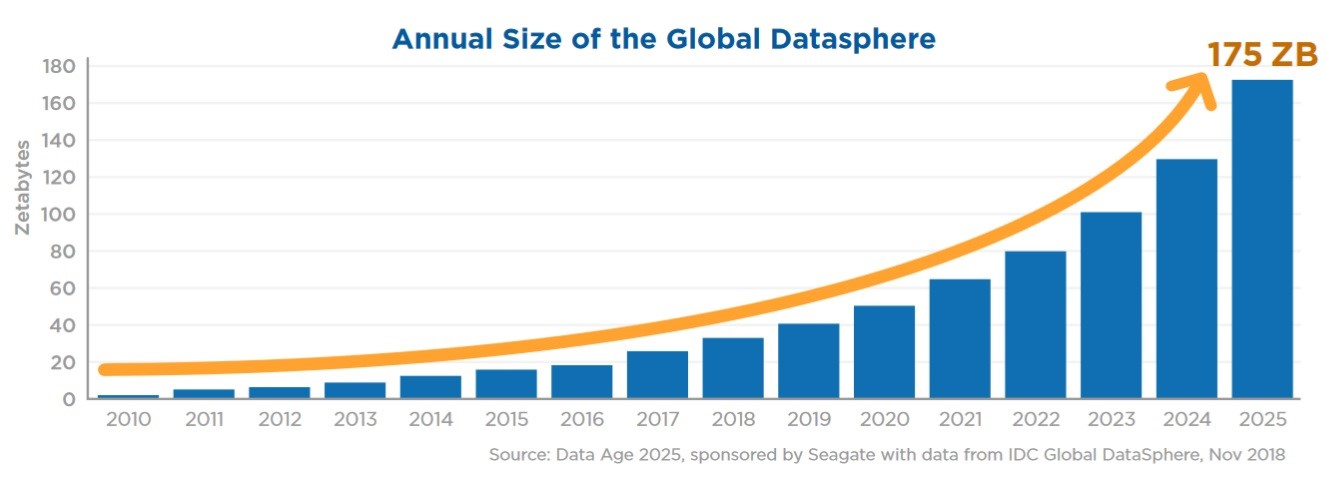
\includegraphics[width=1\textwidth]{images/annual_datasphere_growth.jpg}
    \caption{Annual Global Datasphere Size, Estimated by \acrshort{idc}}
    \label{fig:datasphere_growth}
\end{figure}

\section{Background}
In this chapter the terms and concepts that are necessary for understanding the thesis will be defined. 

\subsection{Recommender System}
\label{subsec:rec_sys}
A recommender system is an information retrieval system that aims to predict the rating of a user for a given item based either on historical rating data or explicit constraints by the user \cite{aggarwal2016recommender}.
The historical data can either be \textit{implicit} i.e. users in the system do not explicitly give ratings to items (e.g. clicks) or the data
can be \textit{explicit} i.e. users in the system provide explicit ratings for items.\\
A basic distinction is made between the following three types of recommender systems:
\begin{enumerate}
    \item Content - based recommender systems 
    \item \acrfull{cf} recommender systems
    \item Knowledge - based recommender systems
\end{enumerate}

\noindent Content - based recommender systems exploit the attributes of items to make their recommendations.
This means that items are interpreted as similar if their attribute - values are similar. 
In content - based recommender systems the item - similarity is combined with the historical user - data to produce recommendations.
For this purpose a similarity - matrix ${A} \in \mathbb{R}^{n \times n}$ (with $n$ being the number of items) is calculalated to find
similar items. The assumption that a content - based recommender system makes is that the ratings of one specific user strongly
correlate for similar items.

\noindent Collaborative filtering recommender systems exploit the similarity of users to make their recommendations. Only
implicit or explicit feedback provided by the users is used in this case. The goal is to find clusters of similar users i.e.
users whose rating - behaviour is similar. The assumption that a \acrshort{cf} recommender system makes is that
unspecified ratings can be imputed because the ratings of similar users for the same items strongly correlate.

\noindent Knowledge based recommender systems are often used for items that are not purchased often and are available in many different combinations of options, e.g. real estate or automobiles. Therefore it may be the case that sufficient ratings are not available to provide a recommendation to a user. In this case the user provides explicit constraints about the properties of an item which the recommender system uses to find suitable items. Knowledge based recommender systems are the only type of recommender systems that allow the user to explicitly specify which items they want.

\subsection{Similarity Measures in Recommender Systems}

A binary similarity measure is defined as \begin{equation}
    f\colon\mathbb{R}^{n}\times\mathbb{R}^{n}\to [0,1]
\end{equation}
It maps the n - dimensional representation of two objects to a similarity value in the range [0,1]. A similarity value of 0 indicates that there is no similarity between the two objects while a similarity value of 1 indicates that the two items are identical. 
A binary similarity measure that will be used in this thesis is the \textit{cosine similarity}, which is defined as
\begin{center}
\begin{equation}
    \text{cos}(A, B) = \frac{A.B}{\|A\|\|B\|}
\end{equation}
\end{center}
with $A, B \in\mathbb{R}^{n}$. For $\|A\| = \|B\| = 1$ the \textit{cosine similarity} is equal to the \textit{dot product}.

\subsection{Matrix Factorization}
A matrix factorization decomposes a given matrix ${A} \in {\mathbb{R}}^{n \times m}$ into the product ${B} \text{\mathbf{C}}^\top$ of two lower - dimensional matrices $B \in\mathbb{R}^{n \times d}$ and $C \in \mathbb{R}^{m \times d}$.
In the context of recommender systems each cell $c_i_j$ of matrix $A$ represents the feedback of user $u_i$ for item $i_j$.
Each row of the lower - dimensional matrix $B$ is the $d$ - dimensional representation of a user. Likewise, each row of the lower - dimensional matrix $C$ is the $d$ - dimensional representation of an item.
The higher the dimension $d$, the more latent features of an item are found that a user can either like or dislike. 
Usually it holds that $d \ll n,m$.
The goal of a matrix factorization is to approximate the original matrix $A$ by the product of the low - dimensional matrix $B$ and the
transposed low - dimensional matrix ${C}^\top$:
\begin{center}
\begin{equation}
A \approx BC^\top
\end{equation}
\end{center}
The concept is illustrated in Figure \ref{fig:mf_schema}.
\begin{figure}[ht]
    \centering
    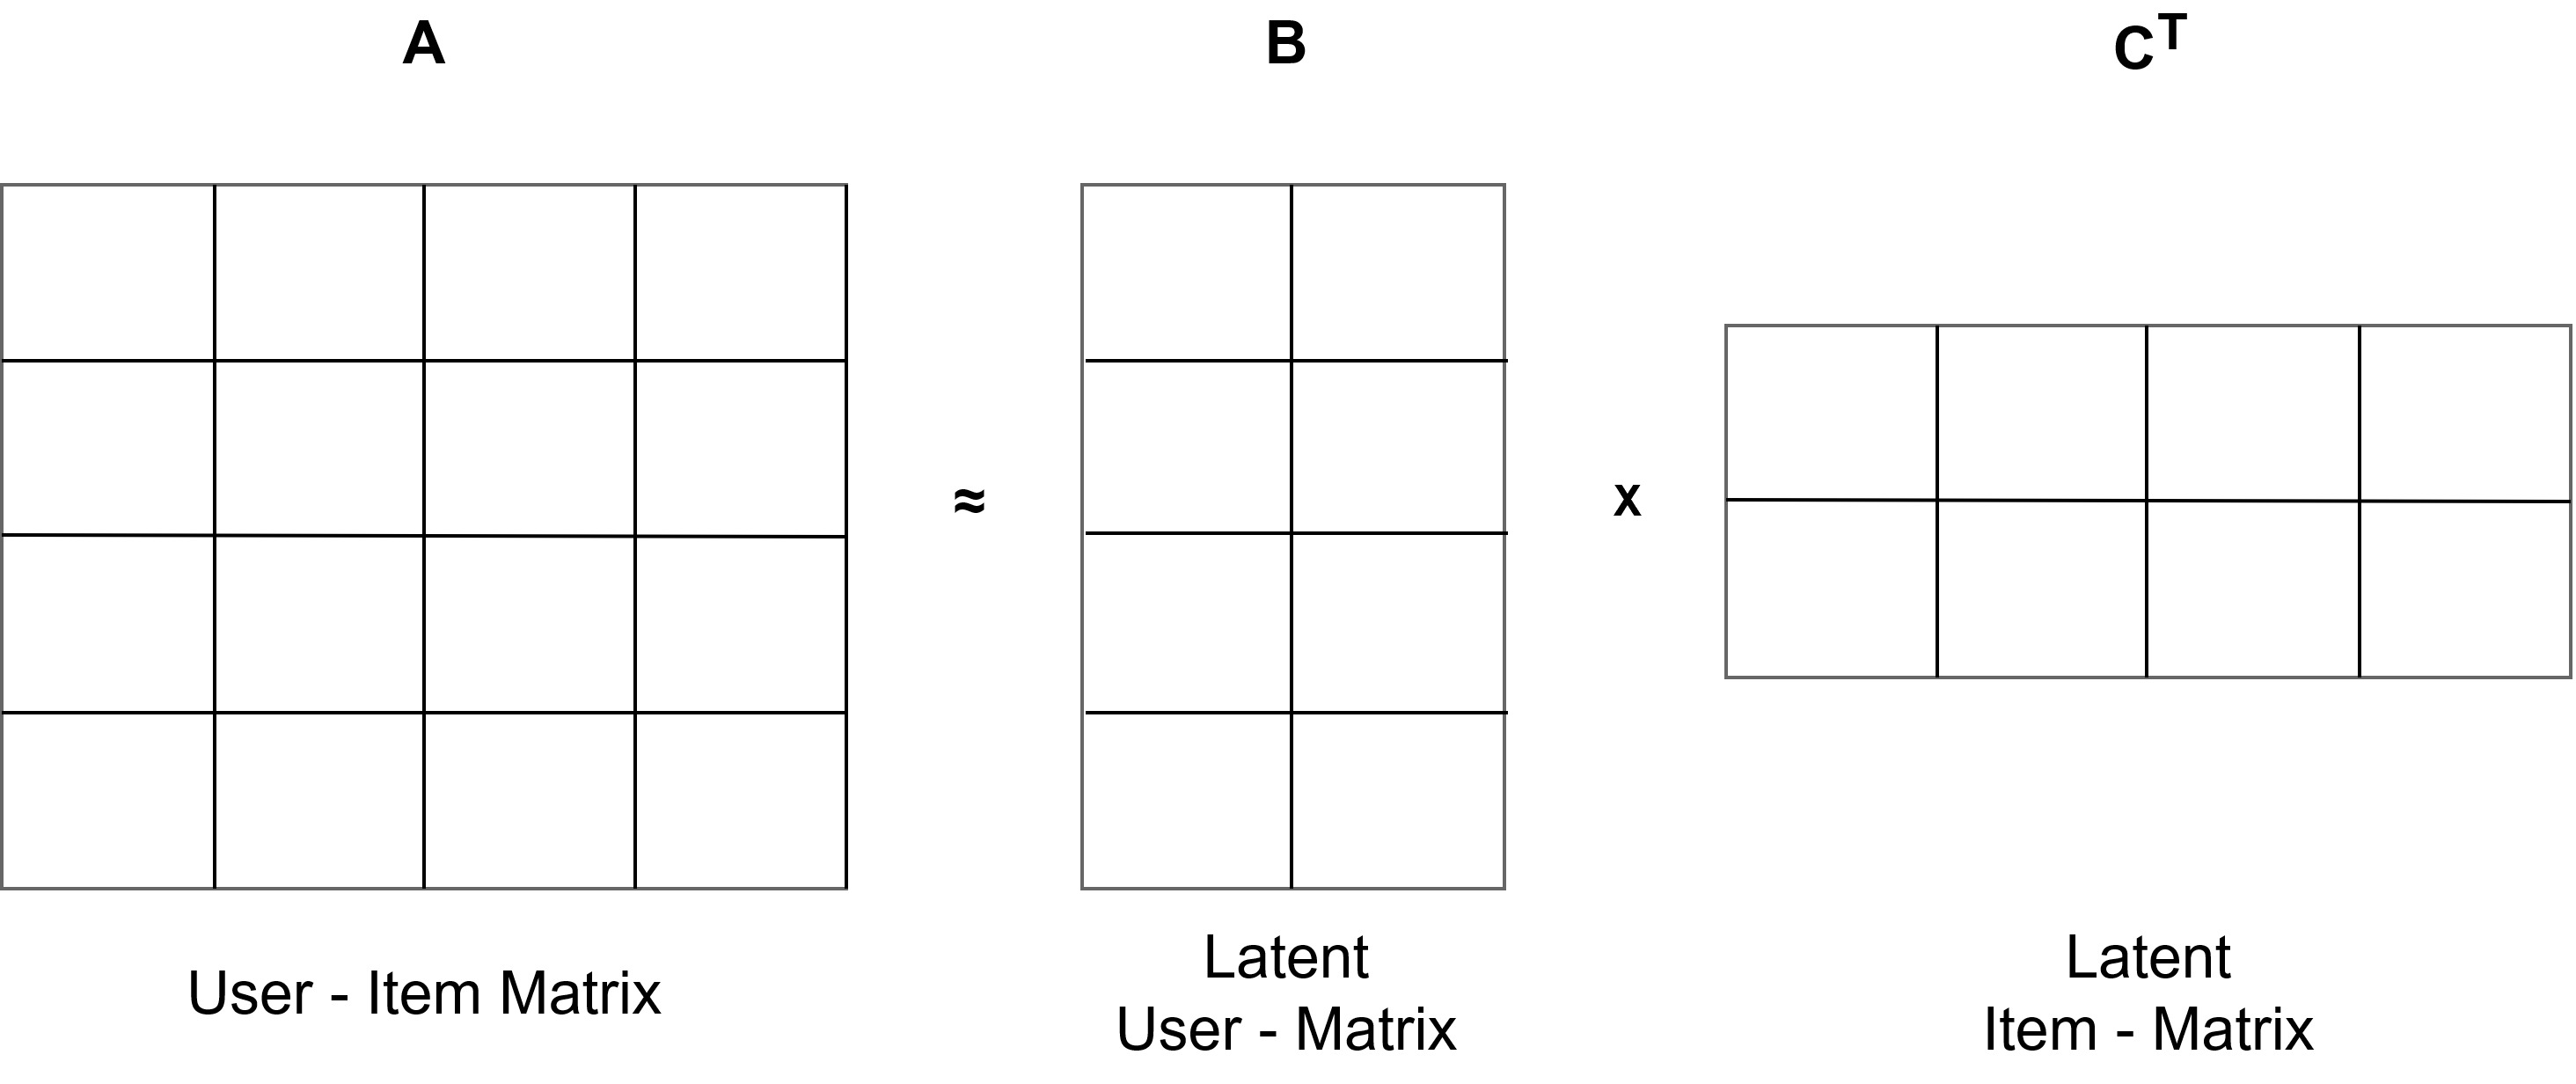
\includegraphics[width=1\textwidth]{images/matrix_factorization}
    \caption{Matrix Factorization Schema With Embedding Dimension d = 2}
    \label{fig:mf_schema}
\end{figure}

\subsection{Perceptron}
The perceptron is a simple mathematical model that performs a dot - product of $n$ inputs $x_1, .., x_n \in \mathbb{R}$, $n$ weights $w_1, .., w_n \in \mathbb{R}$ and a bias term $b \in \mathbb{R}$ \cite{rosenblatt1958perceptron}. The result of the dot - product is then fed into an activation - function whose output decides if this perceptron is activated or not, taking on a binary value. This activation function was originally the Heaviside step function, which is defined as:\\
\begin{equation}
        H(x) = \left\{
	\begin{array}{ll}
		\text{1} & \mbox{if } x \geq 0\\
		\text{0} & \mbox{if } x < 0 \\
	\end{array}
\right.
    \end{equation}
The perceptron model is illustrated in Figure \ref{fig:perceptron}.

\begin{figure}[ht]
    \centering
    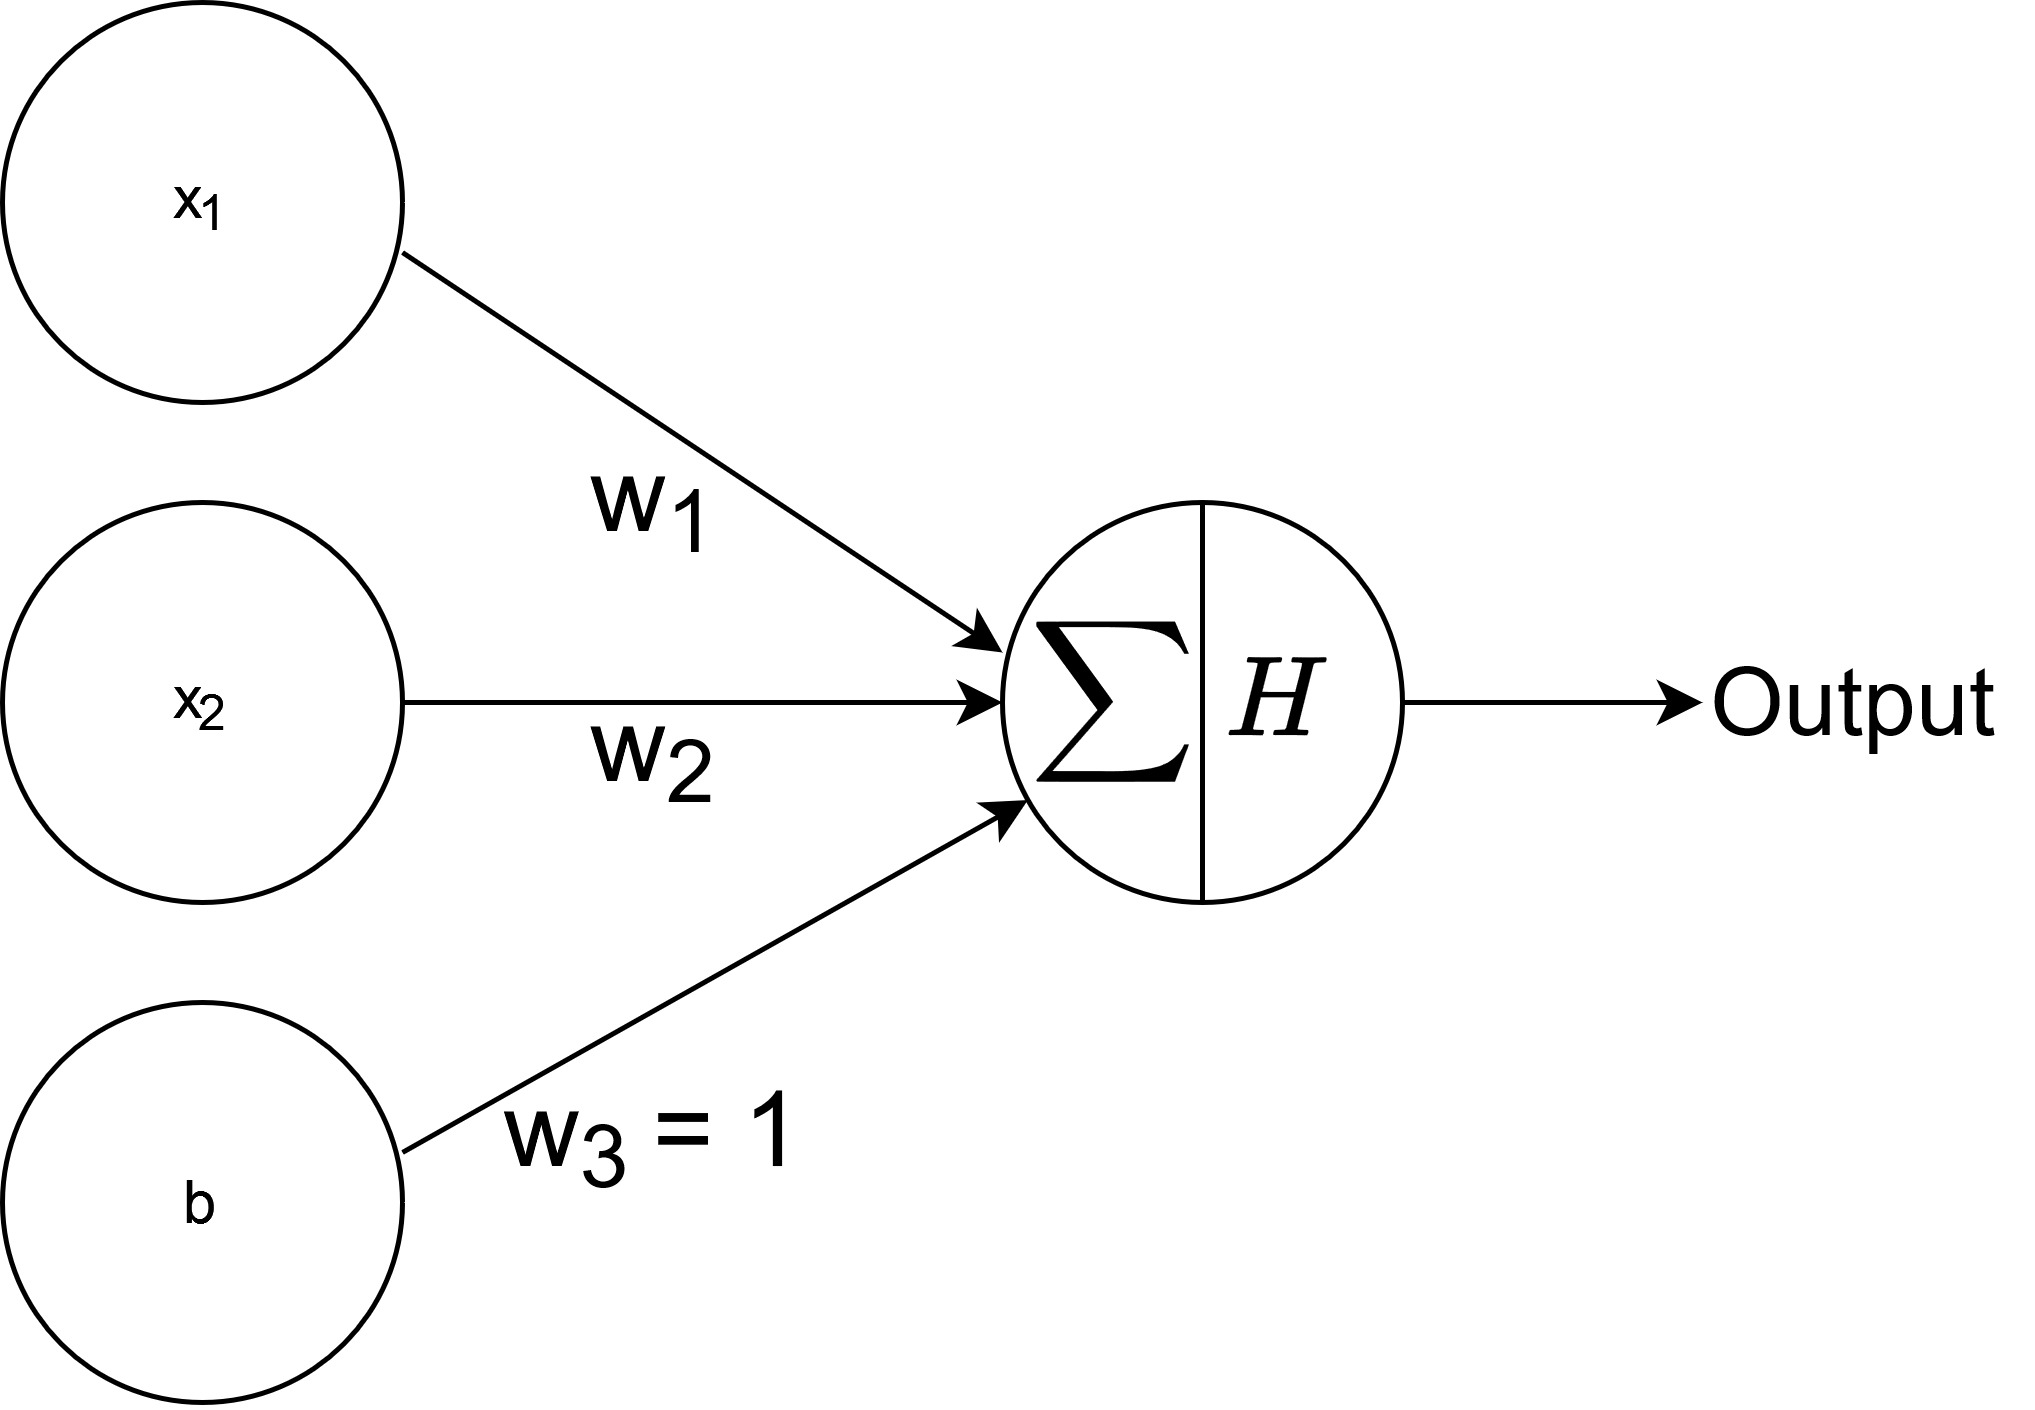
\includegraphics[scale=0.12]{images/perceptron.jpg}
    \caption{Perceptron Schema With $n=2$}
    \label{fig:perceptron}
\end{figure}

\subsection{Neural Network}
A neural network is a mathematical model that is able to approximate any mathematical function in order to map a d - dimensional input to a k - dimensional output. To achieve this, linear and non - linear transformations are applied alternately to the input. A neural network consists of an input layer, arbitrary many hidden layers and one output layer. The neurons in the hidden layer are perceptrons with a specific activation function that is identical for each layer.\\
As a single perceptron can only model linear functions due to the linear nature of the dot - product, non - linear activation functions are applied to the output of each perceptron in the hidden layers. This way, a neural network is able to approximate any mathematical function, not only linear functions. In fully connected neural networks there is a weight specified for each neuron - pair combination of two adjacent layers. All these weights compose the learnable parameters $\theta$, whose optimal values are iteratively updated by the backpropagation algorithm in an unsupervised manner \cite{rumelhart1986learning}. A fully connected neural network is illustrated in Figure \ref{fig:nn}.

\begin{figure}[ht]
    \centering
    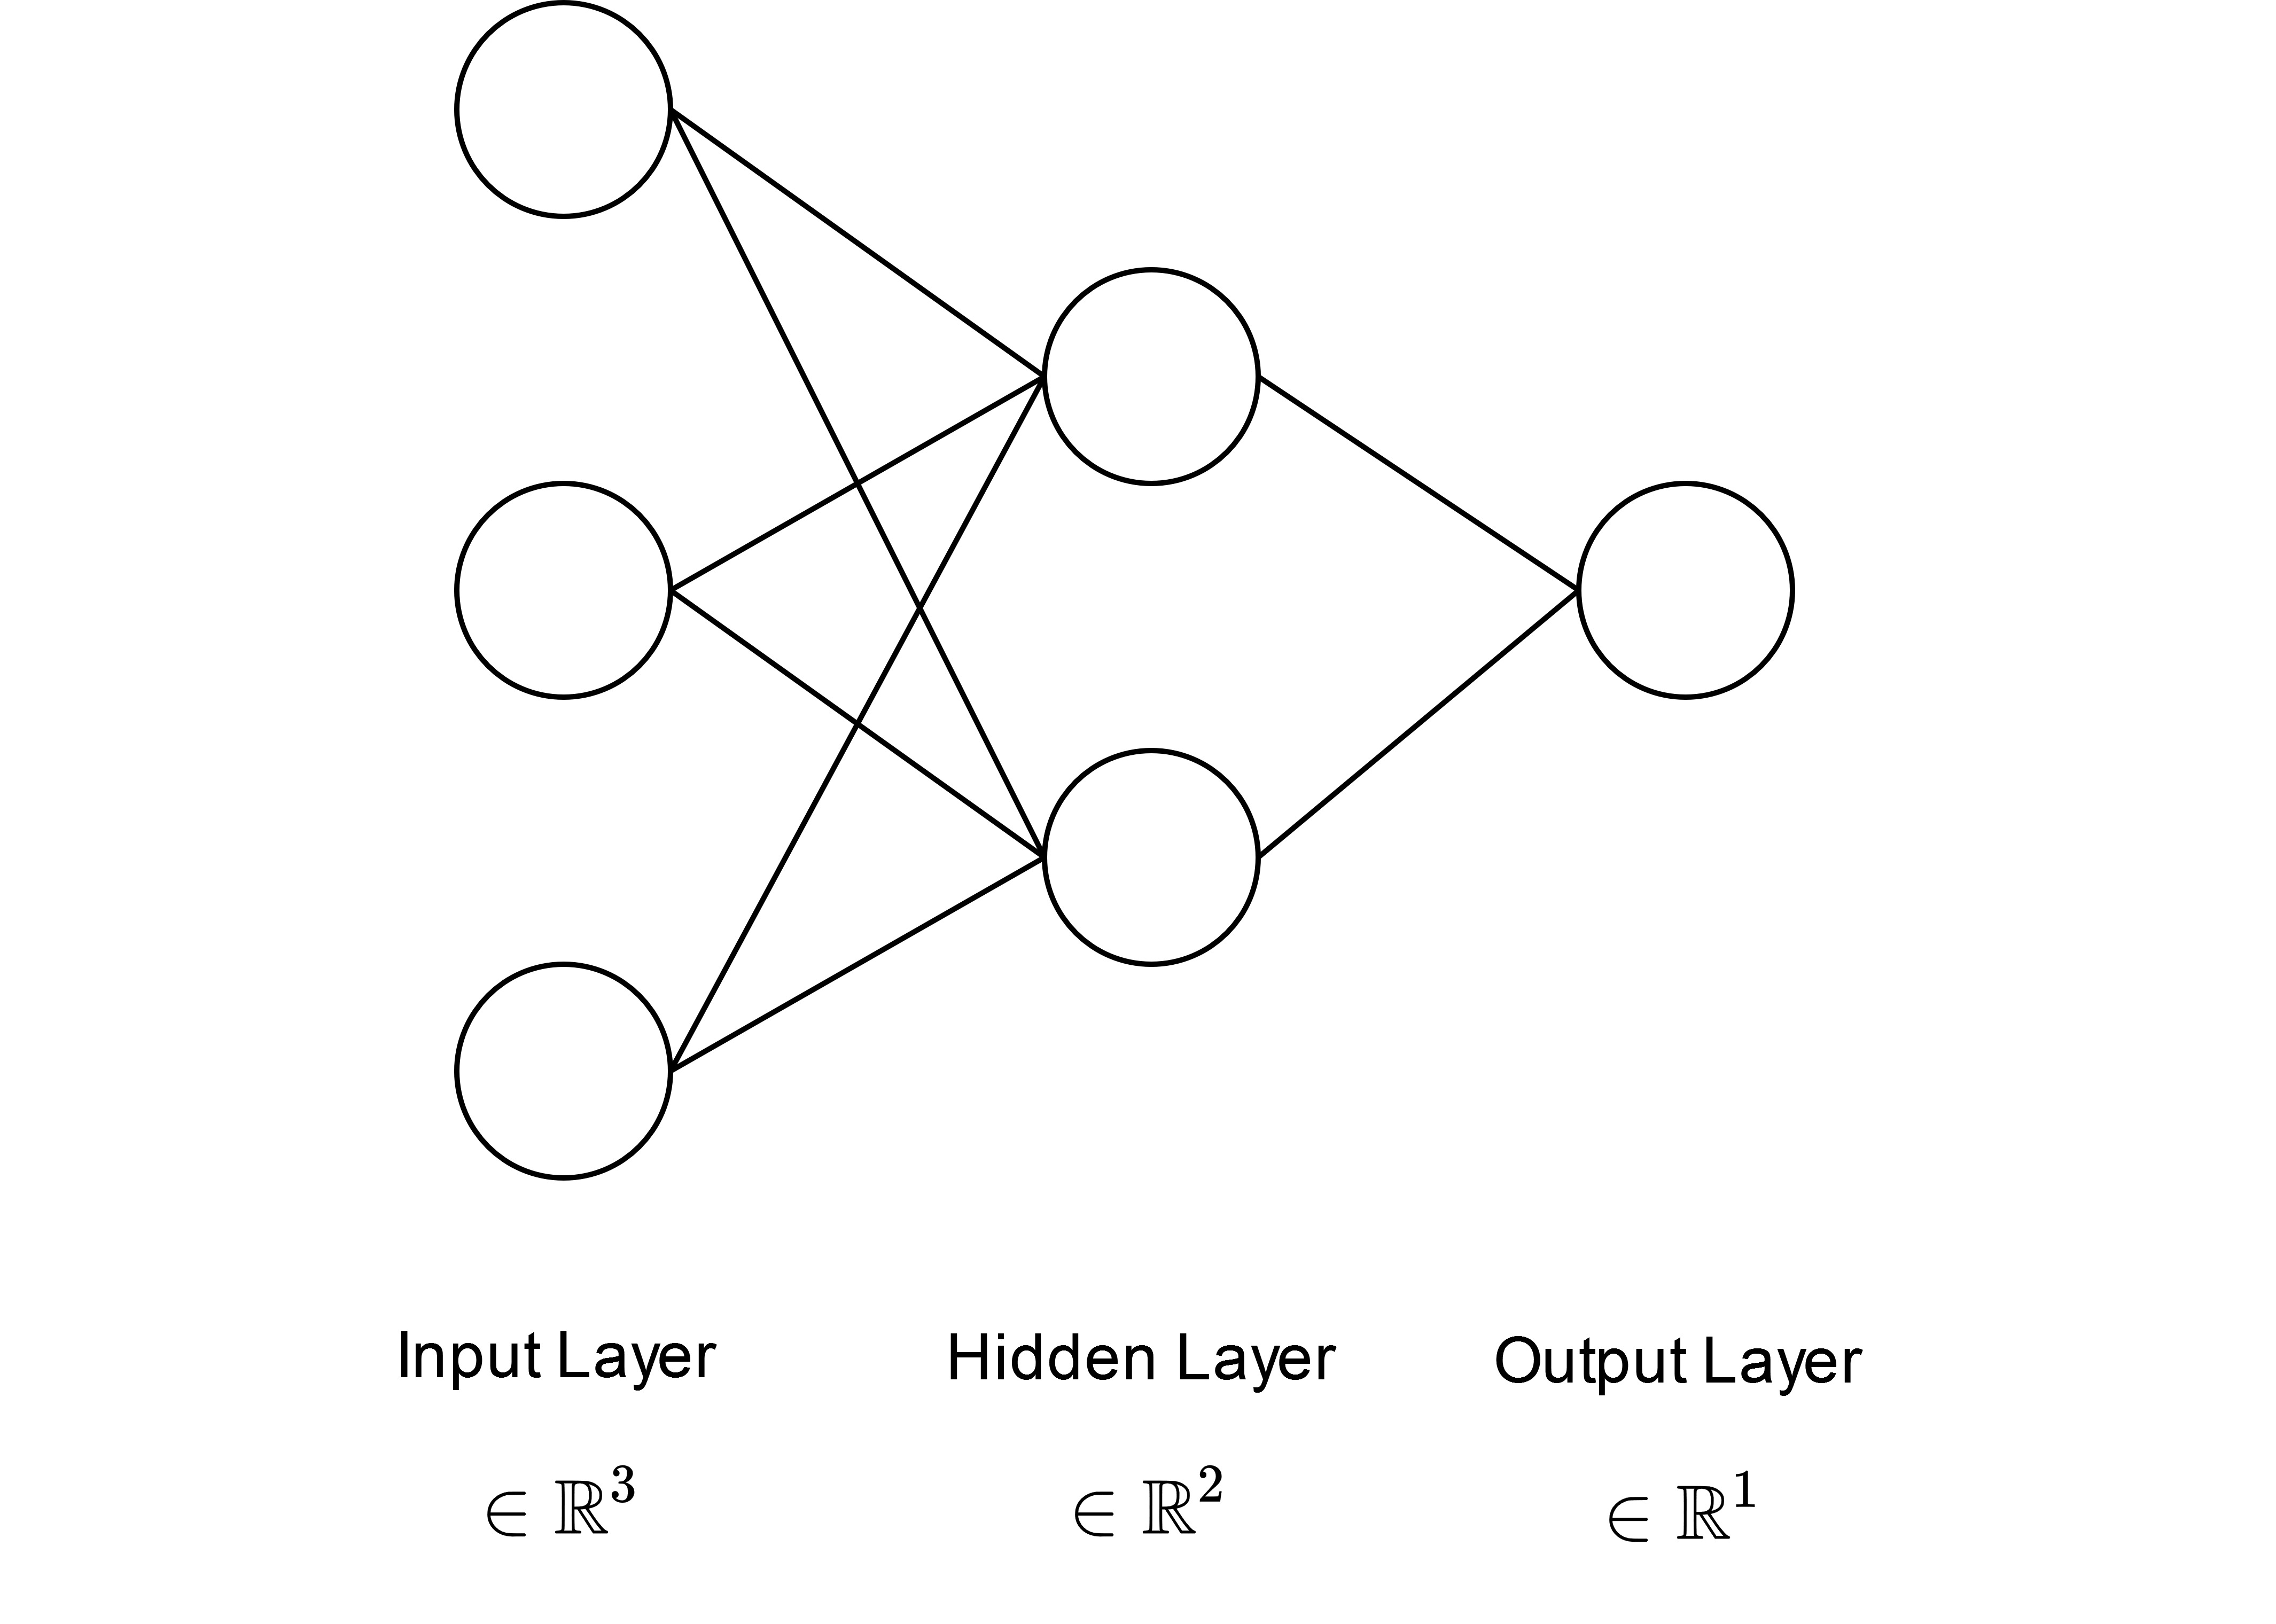
\includegraphics[width=1\textwidth]{images/nn.jpg}
    \caption{Fully Connected Neural Network With $d=3$, $k=1$ and One Hidden Layer.}
    \label{fig:nn}
\end{figure}

\subsection{Autoencoder}
\label{chap:autoencoder}
An autoencoder is typically a neural network with one input layer, one hidden layer and one output layer \cite{bank2021autoencoders}.
Autoencoders are often applied for dimensionality reduction. That is, reducing the high dimensional representation of the input into a low dimensional representation from which the original input can be approximated.\\
The step of mapping the input to the low dimensional representation (encoding) is referred to as the encoder step. Similarly, the step of mapping the encoding to an approximation of the input is called the decoding step.\\
The low dimensional representation is learned in an unsupervised way by trying to regenerate the input from the encoding.

\subsection{Transformer}
The transformer model is composed of an encoder - decoder architecture and fully connected neural networks that are combined with the concept of self - attention \cite{vaswani2017attention}. The transformer model is the predominant model for solving natural language processing tasks. The introduction of the transformer model led to the development of the transformer - based language model \acrfull{bert} by Google \cite{devlin2018bert}. \acrshort{bert} reached new state - of - the - art performances on a number of \acrfull{nlp} tasks and its' performance is often used as a benchmark to evaluate new \acrshort{nlp} models.

\subsection{\acrfull{tfidf}}
In information retrieval the \acrshort{tfidf} - metric is used to compute the importance of a term in a corpus of texts w.r.t. to a search query in order to retrieve the most relevant documents for this query \cite{jones1972statistical}.\\
The \acrshort{tfidf} is defined as
\begin{center}
\begin{equation}
    \text{\acrshort{tfidf}(t, d, D)} = \text{tf(t,d)} \cdot \text{idf(t,D)}
\end{equation}
\end{center}
where tf is the term - frequency and idf the inverse document - frequency.\\
t is a specific term, d is a specific document with $d \in D$ where $D$ is the set of all documents within the corpus.\\
Let 
\begin{equation}
    \sum\limits_{t \in d}f_{t,_d} = \text{total}(d)
\end{equation} 
$f_t,_d$ calculates the number of times the term $t$ occurs in $d$.\\
The term - frequency is defined as 
\begin{center}
\begin{equation}
    \text{tf(t,d)} = \frac{f_t,_d}{\text{total}(d)}
\end{equation}
\end{center}
\noindent The inverse document - frequency is defined as:
\begin{center}
\begin{equation}
    \text{idf}(t,D) = \text{log}(\frac{|D|}{\sum\limits_{d \in D}\mathbbm{1_{d}}(t)}}})
\end{equation}
\end{center}
where $\mathbbm{1_{d}}(t)$ is the \textit{indicator function} of term $t$ being in document $d$. 
\subsection{Classification Metrics for Imbalanced Data Sets}
\label{sec:metrics}
The most frequently used metric when evaluating a binary classification problem is the \texit{accuracy} metric. It is defined as the ratio of correctly classified instances to the number of all instances. In binary classifications the two class labels are called majority class and minority class with the majority class being the more frequent class. To define accuracy the following concepts are needed
\begin{itemize}
    \item \acrfull{tp}: Minority class is correctly predicted.
    \item \acrfull{fp}: Minority class is wrongly predicted.
    \item \acrfull{tn}: Majority class is correctly predicted.
    \item \acrfull{fn}: Majority class is wrongly predicted.
\end{itemize}
These metrics are well - established to characterize and evaluate a binary classification \cite{tharwat2020classification}. \\
The accuracy is defined as:
\begin{equation}
    \text{Accuracy} = \frac{\acrshort{tp} + \acrshort{tn}}{\acrshort{fp} + \acrshort{fn} + \acrshort{tp} + \acrshort{fn}}
\end{equation}\\
The accuracy metric does not take the label distribution within the data into consideration and can therefore be easily misleading. A majority classifier evaluated on a data set with a label distribution of 5 percent minority class labels and 95 percent majority class labels will for example reach 95 percent accuracy.\\
Thus, in cases of imbalanced data sets the accuracy metric is not a reasonable metric to use.\\
Four metrics that do take the label distribution into account which are mentioned in the literature are the \texit{F - Score}, the \texit{G - Mean}, \texit{Recall} and \texit{Precision} \cite{he2009learning}.\\
In the following the minority class will be the positive class and the majority class will be the negative class.\\ 
Too define the F - Score and the G - Mean, Recall and Precision need to be defined:\\
\begin{equation}
    \text{Recall} = \frac{\acrshort{tp}}{\acrshort{tp} + \acrshort{fn}}
\end{equation}
\begin{equation}
    \text{Precision} = \frac{\acrshort{tp}}{\acrshort{tp} + \acrshort{fp}}
\end{equation}\\
Incorporating Recall and Precision, the F - Score is defined as:\\
\begin{equation}
    \text{F - Score} = \frac{(1 + \beta)^{2} \cdot \text{Recall} \cdot \text{Precision}}{\beta^{2} \cdot \text{Recall} + \text{Precision}}
\end{equation}
where $\beta$ is a parameter that controls the relative importance of precision versus recall. If precision and recall should be taken into account equally, then $\beta = 1$.\\
The G - Mean is defined as:\\
\begin{equation}
    \text{G - Mean} = \sqrt{\frac{\acrshort{tp}}{\acrshort{tp} + \acrshort{fn}} \cdot \frac{\acrshort{tn}}{\acrshort{tn} + \acrshort{fp}}}
\end{equation}
These four metrics are designed for binary classification problems where there are only two labels. In order to map these metrics to classification problems where the number of labels is greater than two, the following two approached can be applied. They will be illustrated for the F - Score metric:
\begin{enumerate}
    \item Taking the average F - Score per class $c$, where $c$ is the minority class and all other classes are the majority class. The set of all classes is denoted as $C$. The advantage is that all labels are treated as equally important:
    \begin{equation}
        \text{F - Score}_A = \frac{1}{|C|}\sum_{c \in C} \text{F - Score}_c
    \end{equation}
    \item Take the weighted average F - Score per class $c$, where $c$ is again the minority class and whose weight $w$ is its' share of the total number of ratings:
    \begin{equation}
        \text{F - Score}_W = \sum_{c \in C} w_c \cdot \text{F - Score}_c , \;\;\sum_{c \in C} w_c = 1
    \end{equation}
    The disadvantage is that this gives again more weight to the more frequent labels. Thus, the first approach will be used later in the evaluation process.
\end{enumerate}
The G - Mean, Recall and Precision can be adapted in the same way to the multivariate classification problem with the number of labels $n > 2$. 

\section{Data Set}
The data set consists of ratings of arguments on two different topics from German food policy: The prohibition of plastic packaging and the prohibition of genetic engineering \cite{brenneis2021will}. The ratings for these arguments were given by German online participants. The collection of data was conducted at three different time points: August 2020 ($T_1$), October 2020 ($T_2$) and December 2020 ($T_3$). 

\subsection{Subdivision of the Data Set}
\label{chap:subdivison}
The data set is divided into two different time transitions. The first one is defined as $T_1 \xrightarrow[]{} T_2$ and the second one is defined as $T_2 \xrightarrow[]{} T_3$.\\
The \acrshort{poc} and the \acrshort{pow} tasks are defined on both time transitions.
Each of these time transitions is split into train, validation and test data sets with the ratio $60\%, 20\%, 20\%$. \\
The data sets can be further divided into the \acrshort{poc} and \acrshort{pow} task. The conviction columns are binary columns in $\{0,1\}$ and the weight columns take values from $\{0,1,2,3,4,5,6\}$. While the conviction columns indicate if a user is convinced by a given argument or not, the corresponding weight columns indicate how strong the users' conviction regarding the specific argument is.

\subsection{Properties of the Data Set}
In \autoref{tab:my_label} different properties of the data set regarding the subdivisions described in \autoref{chap:subdivison} are presented.

\begin{table}[h!]
    \centering
    \begin{adjustbox}{width=\textwidth}
    \begin{tabular}{|c|c|c|c|c|c|c|c}
    \hline
     & \multicolumn{2}{|c|}{Train} & \multicolumn{2}{|c|}{Validation} &
      \multicolumn{2}{|c|}{Test} \\
     \hline
     \text{Properties} &  
     $T_1 \to T_2$ & 
     $T_2 \to T_3$ &
     $T_1 \to T_2$ & 
     $T_2 \to T_3$ & 
     $T_1 \to T_2$ & 
     $T_2 \to T_3$\\
    \hline
    Instances & 672 & 553 & 144 & 116 & 145 & 113 \\
    \hline
    Sparsity & 90.01\% & 84.13\% & 89.48\% & 81.57\% & 89.46\% & 81.57\% \\
    \hline
    $\mu_c$ & 0.62 & 0.59 & 0.59 & 0.57 & 0.60 & 0.55 \\ 
    \hline
    $\mu_w$ & 3.68 & 3.52 & 3.50 & 3.41 & 3.50 & 3.38\\
    \hline
    $H_c$ & 0.96 & 0.97 & 0.97 & 0.98 & 0.96 & 0.99 \\
    \hline
    $H_w$ & 0.96 & 0.97 & 0.93 & 0.95 & 0.94 & 0.96 \\
    \hline
    \end{tabular}
    \end{adjustbox}
    \caption{Properties of the Provided Data Set}
    \label{tab:my_label}
\end{table}

\noindent $\mu_c$ expresses the mean value of the conviction columns and $\mu_w$ expresses the mean value of the weight columns.\\
$H$ denotes the normalized \texit{Shannon Entropy} and it is used in this case to measure the balance of a data set \cite{shannon1948mathematical}.\\
In this case $H_c$ is the normalized Shannon entropy for the \acrshort{poc} task and $H_w$ is the normalized Shannon Entropy for the \acrshort{pow} task.\\
Given a data set of $N$ instances, $C$ different columns and $M$ possible discrete values that a (user, item) pair can take, the normalized \texit{Shannon Entropy} is defined as follows:
\begin{equation}
    H = \frac{-\sum\limits_{i=1}^{M}\frac{M_i}{N \cdot C} \cdot \text{log} \frac{M_i}{N \cdot c}}{\text{log} M}
\end{equation}

\noindent $M_i$ denotes the number of ratings that were rated with the discrete rating value $i$.\\
\noindent $H=0$ indicates that the data set is completely unbalanced i.e. only one rating is given to each (user,item) pair. $H=1$ indicates that the rating - values are distributed uniformly in terms of occurrences.\\
From \autoref{tab:my_label} it can be observed that the data sets overall are balanced.  Additional to the overall balance of the data set it is of great interest for the modelling as well as for the evaluation to know if the distribution of ratings within a single argument itself is also balanced. Subsection \ref{sec:plots} provides plots as an overview of the rating distribution within single arguments. The ratings for the \acrshort{pow} task are grouped for reasons of clarity.\\
It can be seen from these plots that the distribution of the ratings within single items is highly skewed. As both baseline algorithms rely on the distribution of ratings within specific items, accuracy (\acrshort{poc}) as well as \acrfull{rmse} (\acrshort{pow}) is not a reasonable metric to use in this context. Both metrics do not provide a reliable information about the classifiers' performance with regard to the properties of the data set. Therefore, metrics that take into account the performance on each discrete rating class are more sensible in the context of imbalanced data.\\
In the literature, four of such proposed metrics are the \textit{F - Score}, \texit{G - Mean}, \texit{Precision} and \texit{Recall} \cite{he2009learning}. All metrics are defined in subsection \ref{sec:metrics} and will be used for evaluation of the different models on the different task - / data set - combinations additionally to the provided metrics.

\section{Problem Statement}
Two tasks are defined on the provided data set, the \acrshort{poc} - task and the \acrshort{pow} - task. Within both tasks the challenge is to predict a rating for a user - argument combination in timepoint $T_{a+1}$ with the knowledge of the ratings in timepoint $T_a$.\\ Let $x \in \{0,1,2,3,4,5,6\}^{n}$ denote a partially observed rating - vector of the rating matrix $R \in \mathbb{R}^{m \times n}$, with $m$ being the number of users and $n$ being the number of arguments.
\subsection{Prediction of Conviction (\acrshort{poc})}
The \acrshort{poc} task is defined as follows: given a user, argument pair $(u,i) \in R$, predict the unknown conviction of user $u$ for argument $i$. As this task is a binary classification task, the range of $x$ is limited to $\{0, 1\}$.\\
\subsection{Prediction of Weight (\acrshort{pow})}
The \acrshort{pow} task is defined as follows: given a user, argument pair $(u,i) \in R$, predict the unknown weight of the conviction of user $u$ for argument $i$. This task is a multi classification task, the range of $x$ is $\{0, 1, 2, 3, 4, 5, 6\}$.\\
\subsection{Difficulty of the Tasks}
\label{sec:difficulty}
The difficulty of these tasks is given by the fact that for each user from the test data set in $T_{a+1}$  only two ratings are given in the training data set in $T_{a}$ for each of the respective tasks. Since very little data is available about the relevant users, the available rating information of other users needs to be used to impute the missing values. This setup is defined as a \acrshort{cf} task, as described in \ref{subsec:rec_sys}.\\
\subsection{Generalization of Classification}
CF can be interpreted as a generalization of a classification or regression problem. Traditional classification and regression problems deal with observations $x \in \mathbb{R}^{m}$, where $m - 1$ variables are specified, the independent variables and one variable is unspecified, the dependent variable. The value of the dependent variable needs to be predicted. The independent and dependent variables stay the same throughout all observations. In CF, on the other hand, any variable can be the dependent variable. In addition, more than one of the independent variables may be unspecified. Furthermore, no row - wise split into training data set and test data set can be performed in most cases as any row is likely to contain missing values. The relationship between CF and traditional classification modelling is illustrated in Figure \ref{fig:CFvsClassification}.

\begin{figure}[!ht]
    \centering
    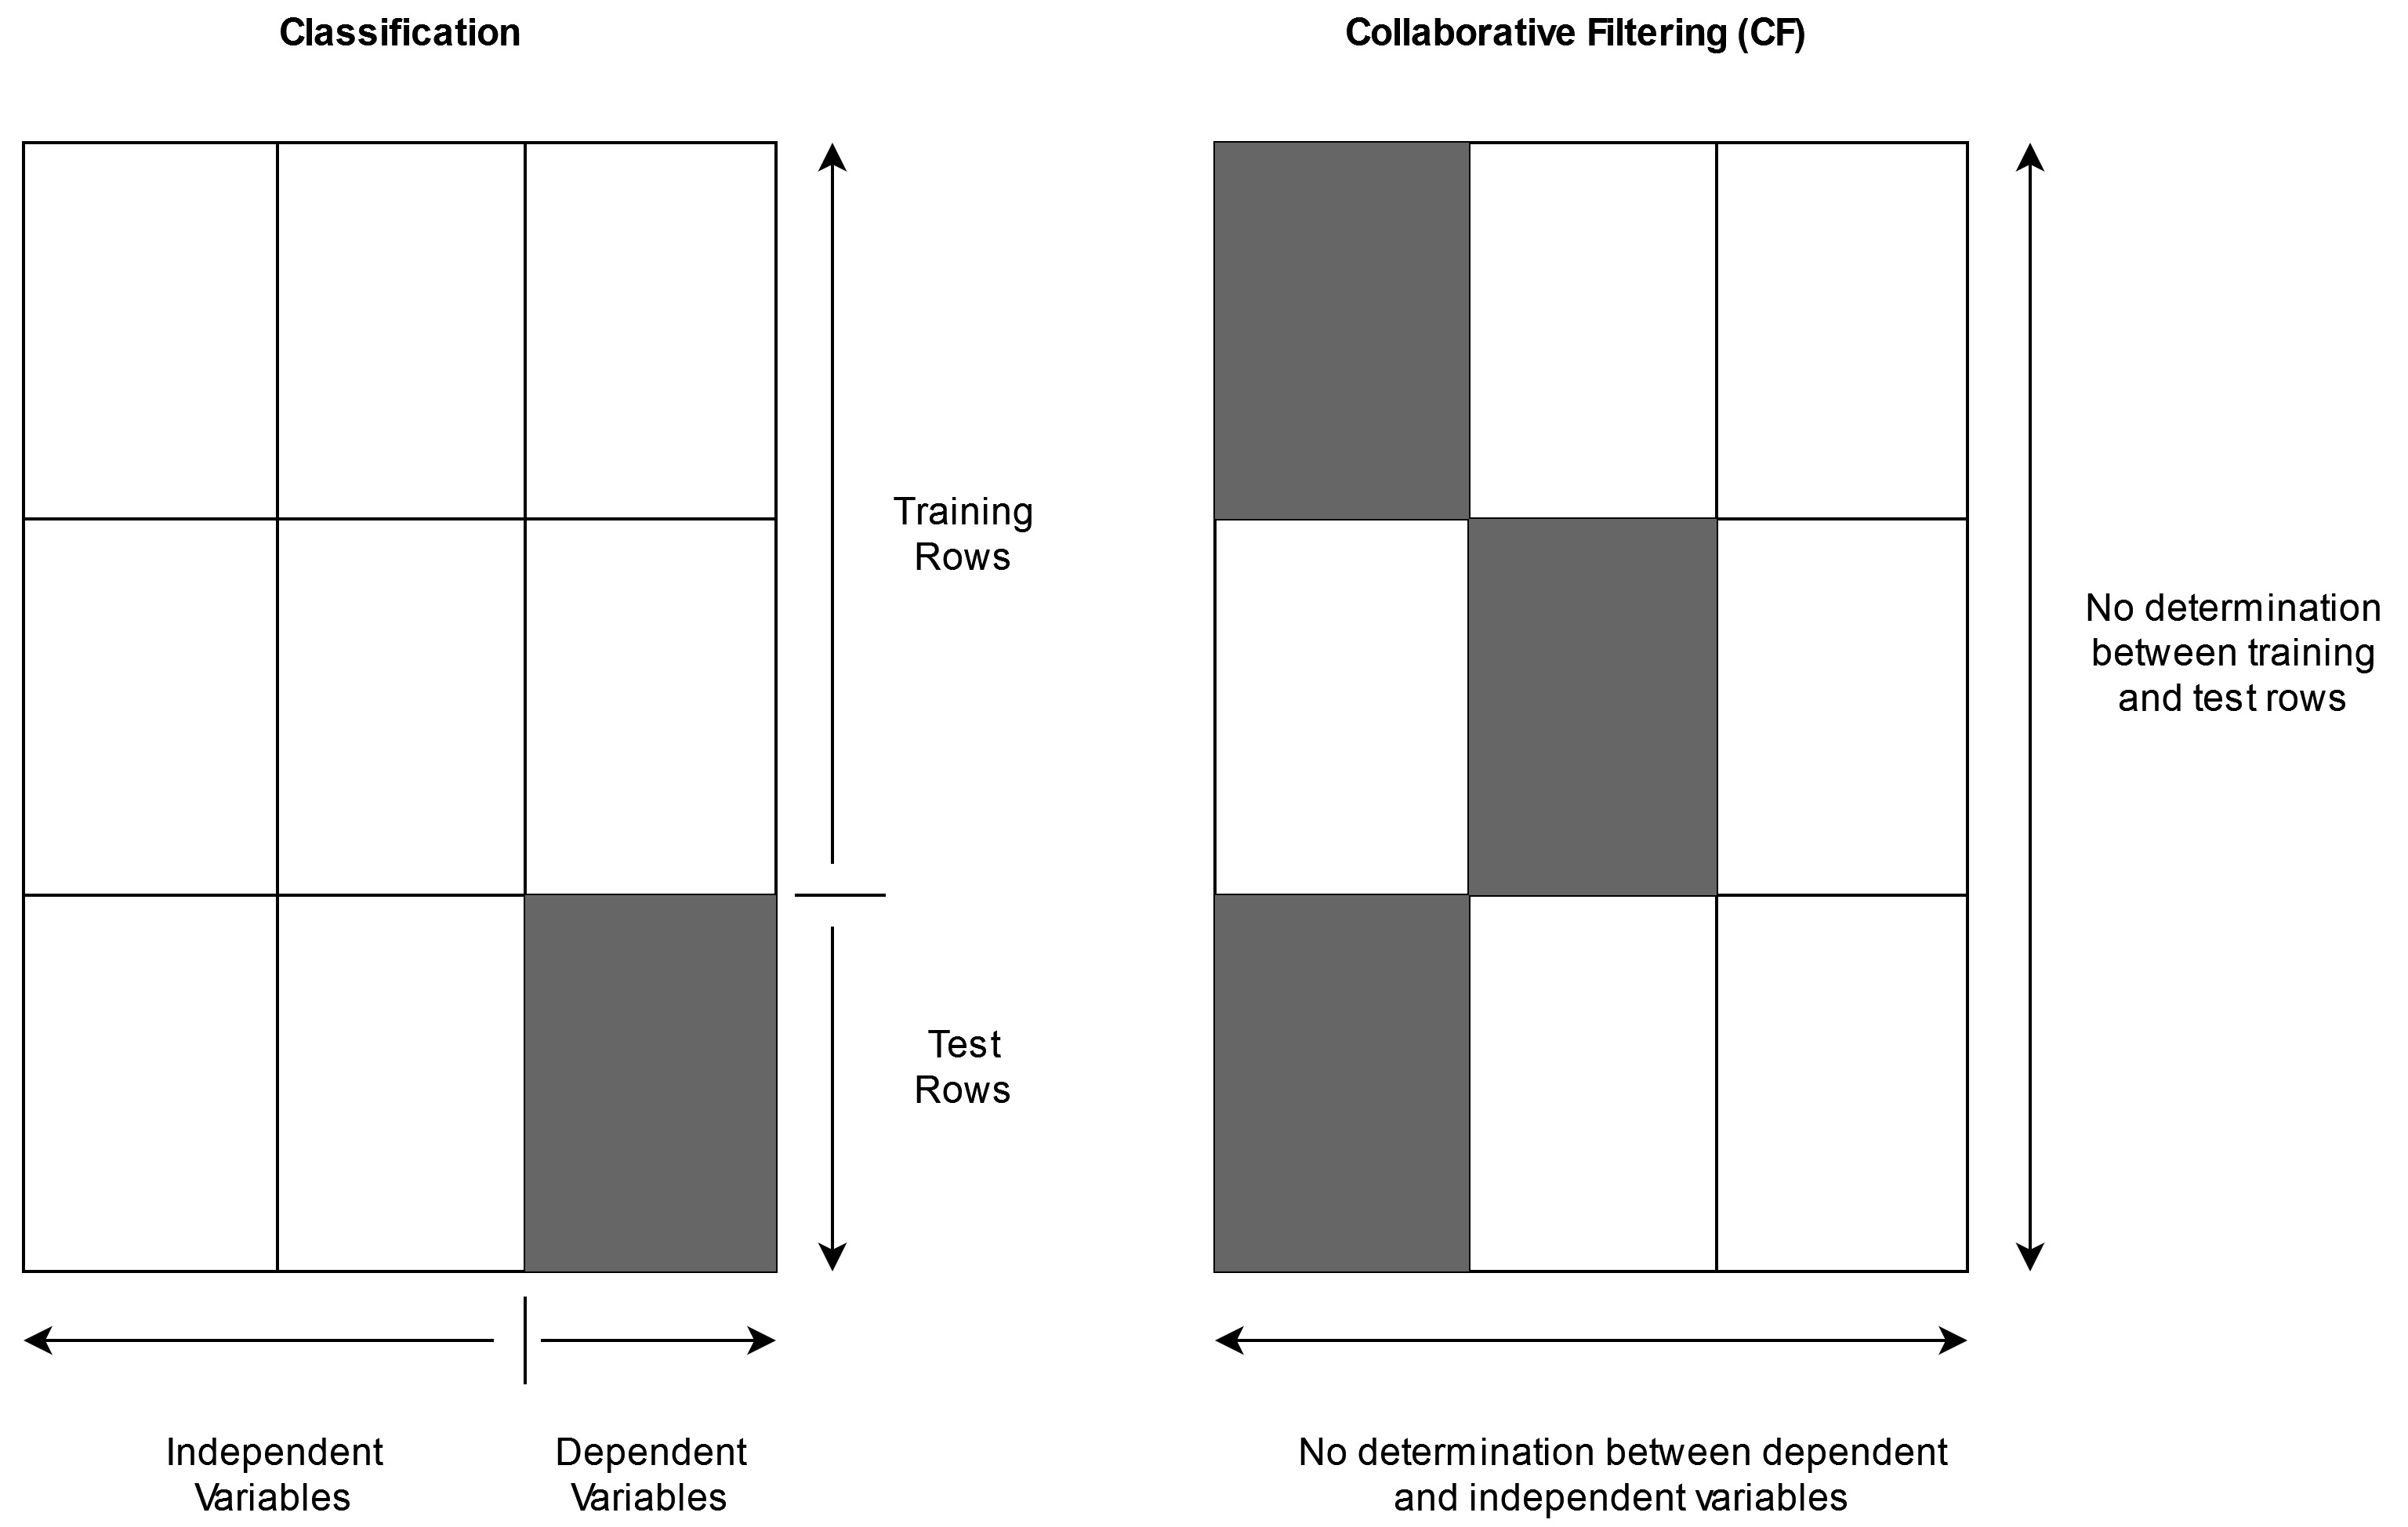
\includegraphics[width=1\textwidth]{images/CFvsClassification2.jpg}
    \caption{Comparison of the Traditional Classification Problem With CF.}
    \label{fig:CFvsClassification}
\end{figure}

\section{Classification Models}

In this section the different approaches that were applied to the classification problem within the provided rating matrix data sets are presented. 

\subsection{\acrfull{tlmf}}
In the following the concept as well as implementation of the \acrshort{tlmf} will be presented.
The \acrshort{tlmf} is a two - step latent factor model which applies two sequential matrix factorizations 
to find the two optimal lower - level matrices whose product approximates the original rating - matrix \cite{li2016two}.
The first matrix factorization computes a similarity matrix of text - entities.
In the context of this thesis these text - entities are arguments. This similarity matrix is then utilized in the second
matrix factorization to include the argument - similarity into the rating prediction additionally to the user - rating information.

\subsubsection{\acrfull{wtmf}}
The first step of the \acrshort{tlmf} is the \acrshort{wtmf}, an unsupervised learning algorithm that has been successfully applied to many natural language processing tasks such as sentence similarity computation \cite{guo2012modeling}. 
The first step in \acrshort{wtmf} is to normalize the arguments, i. e. lemmatizing and lowercasing.
Then a \acrshort{tfidf} - vector is calculated for each normalized argument.
The length of each \acrshort{tfidf} - vector is $|V|$, with $V$ being the vocabulary over all arguments.
The vocabulary $V$ of a text corpus is defined as:
    \begin{equation}
        V = \{T_1 \cup T_2 \cup .. \cup T_n\}    
    \end{equation}
with $T_1, T_2, .., T_n$ being the set of words in the texts $T_1, .., T_n$.\\
For every argument in the corpus, the \acrshort{tfidf} - value for every word in $V$ is calculated. 
The resulting matrix $X$ is called \textit{term - document - matrix}. It contains \acrshort{tfidf} - values of words in each cell. Each argument is represented by a column vector of \acrshort{tfidf} - values for each word in $V$.\\
In the next step $X$ gets approximated by a matrix factorization in order to find lower - dimensional representations of the arguments. $X$ is decomposed into two lower - dimensional matrices $M \in \mathbb{R}^{n \times k}$ and $N \in \mathbb{R}^{m \times k}$.\\ $k$ is the embedding dimension of the sentences and a parameter of the model.
Different from other sentence similarity methods, \acrshort{wtmf} also models the missing words within a text to enrich the features of short texts. The missing words are applied as additional constraints for the semantics of texts.
Since every argument in $X$ is represented in the dimension of $|V|$, many entries in $X$ will be $0$. To account for that fact, a weight - matrix $W  \in \mathbb{R}^{|V| \times |V|}$ 
is introduced to control the influence of cells $x = 0$.\\
Two model parameters $N$ and $M$ are optimized by minimizing the following objective function:
\begin{equation}
\begin{align*}
    L_W = \min_{M,N} \frac{1}{2} W_i_j (X_i_j - M_iN_j^\top) + \frac{\gamma}{2}(\|M\|^2_F + \|N\|^2_F) \\
    W_i_j = \left\{
	\begin{array}{ll}
		1  & \mbox{if } x_i_j \neq 0 \\
		w_m & \mbox{if } x_i_j = 0, w_m \in [0,1]
	\end{array}
\right.
\end{align*}
\end{equation}
In the above objective function $\gamma$ is a free regularization factor that is adjusted to prevent the model from overfitting. $\|\cdot\|^2_F$ is the \textit{Frobenius Norm}.\\

\noindent I will now describe the training process of the \acrshort{WTMF} - model.\\
The model is trained by first initializing the matrices $N$ and $M$ randomly and then updating $N_i$ and $M_j$ iteratively by applying the following equations for every entry $x_i_j \in X$:
    \begin{equation}
        N_i = (M\tilde{W}^{(i)}M^\top + \gamma\mathbb{I})^{-1}B\tilde{W}^{(i)}X^\top_i
    \end{equation}
    \begin{equation}
        M_j =(N\tilde{W}^{(j)}N^\top + \gamma\mathbb{I})^{-1}A\tilde{W}^{(j)}X^\top_j 
    \end{equation}
In the above equations:
\begin{itemize}
    \item $\mathbb{I} \in \mathbb{R}^{k \times k}$  is the \textit{Identity Matrix}
    \item $\tilde{W}^{(i)} \in \mathbb{R}^{n \times n} = \text{diag}(W.,i)$ is a diagonal matrix containing the i - th row of $W$.
    \item $\tilde{W}^{(j)} \in \mathbb{R}^{m \times m} = \text{diag}(W.,j)$ is a diagonal matrix containing the j - th column of $W$.
\end{itemize}
After the training process, the final latent factor matrices $N$ and $M$ have been calculated, such that their product approximates $X$.
$M_j$ now represents the $k$ - dimensional embedding of argument $A_j$.\\
The similarity $Sim(A_i, A_j)$ of two arguments $A_i, A_j$ is now defined as:
    \begin{equation}
        \text{Sim}(A_i, A_j) = \text{cos}(A_i, A_j) = \frac{A_i.A_j}{\|A_i\|\|A_j\|}
    \end{equation}
The pairwise similarity - matrix $S \in \mathbb{R}^{m \times m}$ is defined as:
    \begin{equation}
        S_i_j = \left\{
	\begin{array}{ll}
		\text{Sim}(A_i, A_j)  & \mbox{if } i \neq j\\
		0 & \mbox{if } i=j \\
	\end{array}
\right.
    \end{equation}
The original similarity value of $1$ for $Sim(A_i, A_j)$ with $i=j$ is replaced with $0$ to force the \acrshort{tlmf} model later on to only take into account arguments that differ from the argument at hand when making predictions.\\
$S$ is symmetric, i.e. $\forall{s_i_j} \in S: s_i_j = s_j_i$. Thus, only the entries of an upper triangular matrix need be computed.

\subsubsection{Combining Ratings \& Similarity Matrix}
\label{subsub:tlmf}
The second level of \acrshort{tlmf} attempts to combine the rating matrix with the textual similarity matrix that was computed in the first level into a unified learning model that tries to approximate the given user - argument ratings in the provided data set by applying another matrix factorization.\\
The given rating matrix $Z \in \mathbb{R}^{u \times i}$ is decomposed into two low - dimensional matrices
$Q \in \mathbb{R}^{u\times d}$ and $P \in \mathbb{R}^{i \times d}$. $d$ is the embedding size of the model i.e. each user and each item is represented as an $d$ - dimensional vector.\\
To optimize the model parameters $P, Q$ the regularized squared error is minimized:
\begin{equation}
\begin{align*}
    L_T = \min_{P, Q} \frac{1}{2}\sum\limits_{(u,i) \in K}(Z_u_i - P_uQ_i^\top)^2 + \frac{\lambda}{2}(\|Q\|^2_F + \|P\|^2_F) + \\
    \frac{\alpha}{2}\sum\limits_{i}(q_i - \sum\limits_{j}S_i_j q_j)(q_i - \sum\limits_{j}S_i_j q_j)^\top
\end{algin*}
\end{equation}
The second summand in the above equation is the first regularization. The regularization factor $\lambda$ controls the overfitting of the model to the rating - data.\\
The third summand is the semantic regularization factor. It controls that the argument profiles (i.e. the ratings they get) of similar arguments should be similar. The regularization factor $\alpha$ controls the influence that the semantic relations of the arguments have on the prediction of the model.\\
The set $K$ contains all index - tuples $(u,i)$ of the rating matrix whose value is available.\\
For each $z_u_i \in Z$, $Q_i$ and $P_u$ are updated by the following gradient descent approach:
\begin{equation}
    P_u = P_u + \eta((Z_u_i - P_uQ_i^\top)Q_i - \lambda P_u))
\end{equation}
\begin{equation}
\begin{align*}
    Q_i = Q_i + \eta((Z_u_i - P_uQ_i^\top)P_u - \lambda Q_i) - \\
    \alpha(Q_i - \sum\limits_{j \in \mathbb{N}(i)}S_i_jQ_j) + \\
    \alpha\sum\limits_{j}(S_j_i)(Q_j - \sum\limits_{k \in \mathbb{N}(j)}S_j_k Q_k))
\end{align*}
\end{equation}
In the above equation:
\begin{itemize}
    \item $\eta$ is the \textit{learning rate}. 
    \item $N(i)$ is the \textit{Neighborhood} of argument i. The parameter \textit{n} that is passed to the \acrshort{tlmf} training algorithm determines the number of neighbours (similar arguments) to consider.
\end{itemize}
This training procedure is applied until convergence. Afterwards an unknown value $z_u_i$ can efficiently be predicted by calculating the dot - product P_uQ_i^\top.  

\subsection{\acrshort{bert} + Matrix Factorization}
The similarity matrix of arguments was built by the \acrshort{wtmf} model in the \acrshort{tlmf} model. In this model the similarity matrix is computed by applying a pretrained \acrshort{bert} model to the arguments. Specifically, the \acrshort{bert} - Base model with 12 transformer blocks, 768 hidden layers and 12 self - attention heads is used. This \acrshort{bert} model maps an input sequence to a $768$ - dimensional, dense vector. This mapping is done in such a way that semantically similar sequences are close to each other in the embedding space. The pairwise argument similarity is then computed as the cosine similarity of the normalized argument embeddings.\\
The second step of this model is equal to the second step in the \acrshort{tlmf} model i.e. the computed similarity matrix is incorporated into the matrix factorization model proposed in section \ref{subsub:tlmf}. 

\subsection{AutoRec}
AutoRec is an autoencoder framework specifically designed for \acrshort{cf} tasks \cite{sedhain2015autorec}.
The before described matrix factorization model is a linear latent model, i.e. the complexity of the relationships it is able to model is limited to linear complexity. The goal of implementing the AutoRec model is to model possible non - linear relationships within the rating data and to improve upon the limited predicition power of the matrix factorization model.\\
AutoRec follows the basic architecture of an autoencoder, which is described in section \ref{chap:autoencoder}. AutoRec can either be implemented as an \acrfull{iautorec} or as a \acrfull{uautorec}. In the experiments that were conducted in the paper, the item - based AutoRec yielded better results compared to the user - based AutoRec. It is assumed that this performance difference is caused by the fact that item - vectors are likely to be less sparse than user - vectors in the recommender system scenario.\\
In the following the implementation of \acrshort{iautorec} will be described.\\
Let $x$ denote a partially observed item - vector. The goal of AutoRec is to compute a mapping of the input $x$ into a low - dimensional space from which $x$ can be approximated. Let the reconstruction of the item - vector $x$ be denoted as $h(x;\theta)$. $\theta$ denotes all the learnable parameters of the AutoRec model. The values for the parameters $\theta$ are learned by using backpropagation. The hidden layer size $k \in \mathbb{N}$ is the non - learnable parameter of the AutoRec model. If there are $d$ users in the rating - matrix, then $x \in \{0,1\}^{d}$ for the \acrshort{poc} task and $x \in \{0,1,2,3,4,5,6\}^{d}$ for the \acrshort{pow} task. Let the set of item - vectors be denoted as $I$. The objective function that is optimized upon is given by:
\begin{equation}
    \min_{\theta}\sum_{x \in I} ||x - h(x; \theta)||^{2}_{2}
\end{equation}
where $||x||_{2}^{2}$ denotes the squared Euclidean Norm of a vector $x$.\\
The reconstruction function $h(x, \theta)$ is defined as:\\
\begin{equation}
    h(x,\theta) = f(W \cdot g(Vx + \mu) + b)
\end{equation}
where\\
\begin{itemize}
    \item $f$ and $g$ are activation functions
    \item $W$ and $V$ are weight matrices
    \item $x$ is the (masked) item vector
    \item $\mu$ and $b$ are bias terms
\end{itemize}
$f, g, W$ and $V$ are the learnable parameters $\theta$.\\
To avoid overfitting of the model on the training data, a regularisation term for the weighting matrices is added with $\lambda > 0$:\\
\begin{equation}
   \min_{\theta}\sum_{x \in I} ||x - h(x; \theta)||^{2}_{O} + \frac{\lambda}{2} \cdot (||W||^{2}_{2} + ||V||^{2}_{F})
\end{equation}
The $||\cdot||_{O}$ notation means that only the weights of observed ratings are updated in the AutoRec training procedure.\\
Because the input vector to the network needs to be dense, an appropriate encoding for missing values needs to be found. As the AutoRec model only updates the weights of the network that correspond to observed ratings in the input vector, the missing values can be set to an arbitrary value $\tilde{v} \not\in V$, with $V$ denoting the possible range of rating values. Instead of optimizing the squared distance of the original vector $x$ and its' reconstruction $h(x; \theta)$, the \acrfull{mmse} will be optimized:\\
\begin{equation}
\begin{align*}
    \text{\acrshort{mmse}}(x, h(x;\theta)) = \sum_{u=0}^{d}\frac{\mathbbm{1_{\texit{V}}}(x_u) \cdot (x_u - h(x;\theta)_u)^{2}}
    {\sum_{u=0}^{d} \mathbbm{1_{\texrm{V}}}(x_u)} + \\ \frac{\lambda}{2} \cdot (||W||^{2}_{2} + ||V||^{2}_{F}) 
\end{align*}
\end{equation}
with $\mathbbm{1_{\texrm{V}}}(x_u)$ being the indicator function defined as:\\
\begin{equation}
    \mathbbm{1_{\texrm{V}}}(x_u) = \left\{
	\begin{array}{ll}
		1  & \mbox{if } x_u \in V\\
		0 & \mbox{if } x_u \not\in V \\
	\end{array}
\right.
\end{equation}
This results in the final objective function:\\
\begin{equation}
    \min_{\theta}\sum_{x \in I} \text{\acrshort{mmse}}(x, h(x;\theta)) + \frac{\lambda}{2} \cdot (||W||^{2}_{2} + ||V||^{2}_{F})
\end{equation}
The \acrshort{mmse} is used because the error of the AutoRec model should only be computed over known values in the input vector.\\
The architecture of the AutoRec model is illustrated in \autoref{fig:autorec_example} by a computational graph for an AutoRec instance with input dimension $d = 2$ and hidden layer parameter of size $k=1$. The weights are denoted by $w_{xy}$ where x indicates the position of the weight and y denotes to which input the weight belongs.\\
After learning the optimal values for the learnable parameters $\theta$, a prediction for the combination of user $u$ and item $x$ is produced by:\\
\begin{equation}
    R_u_x = h(x; \theta)_u
\end{equation}

\begin{figure}[!ht]
    \centering
    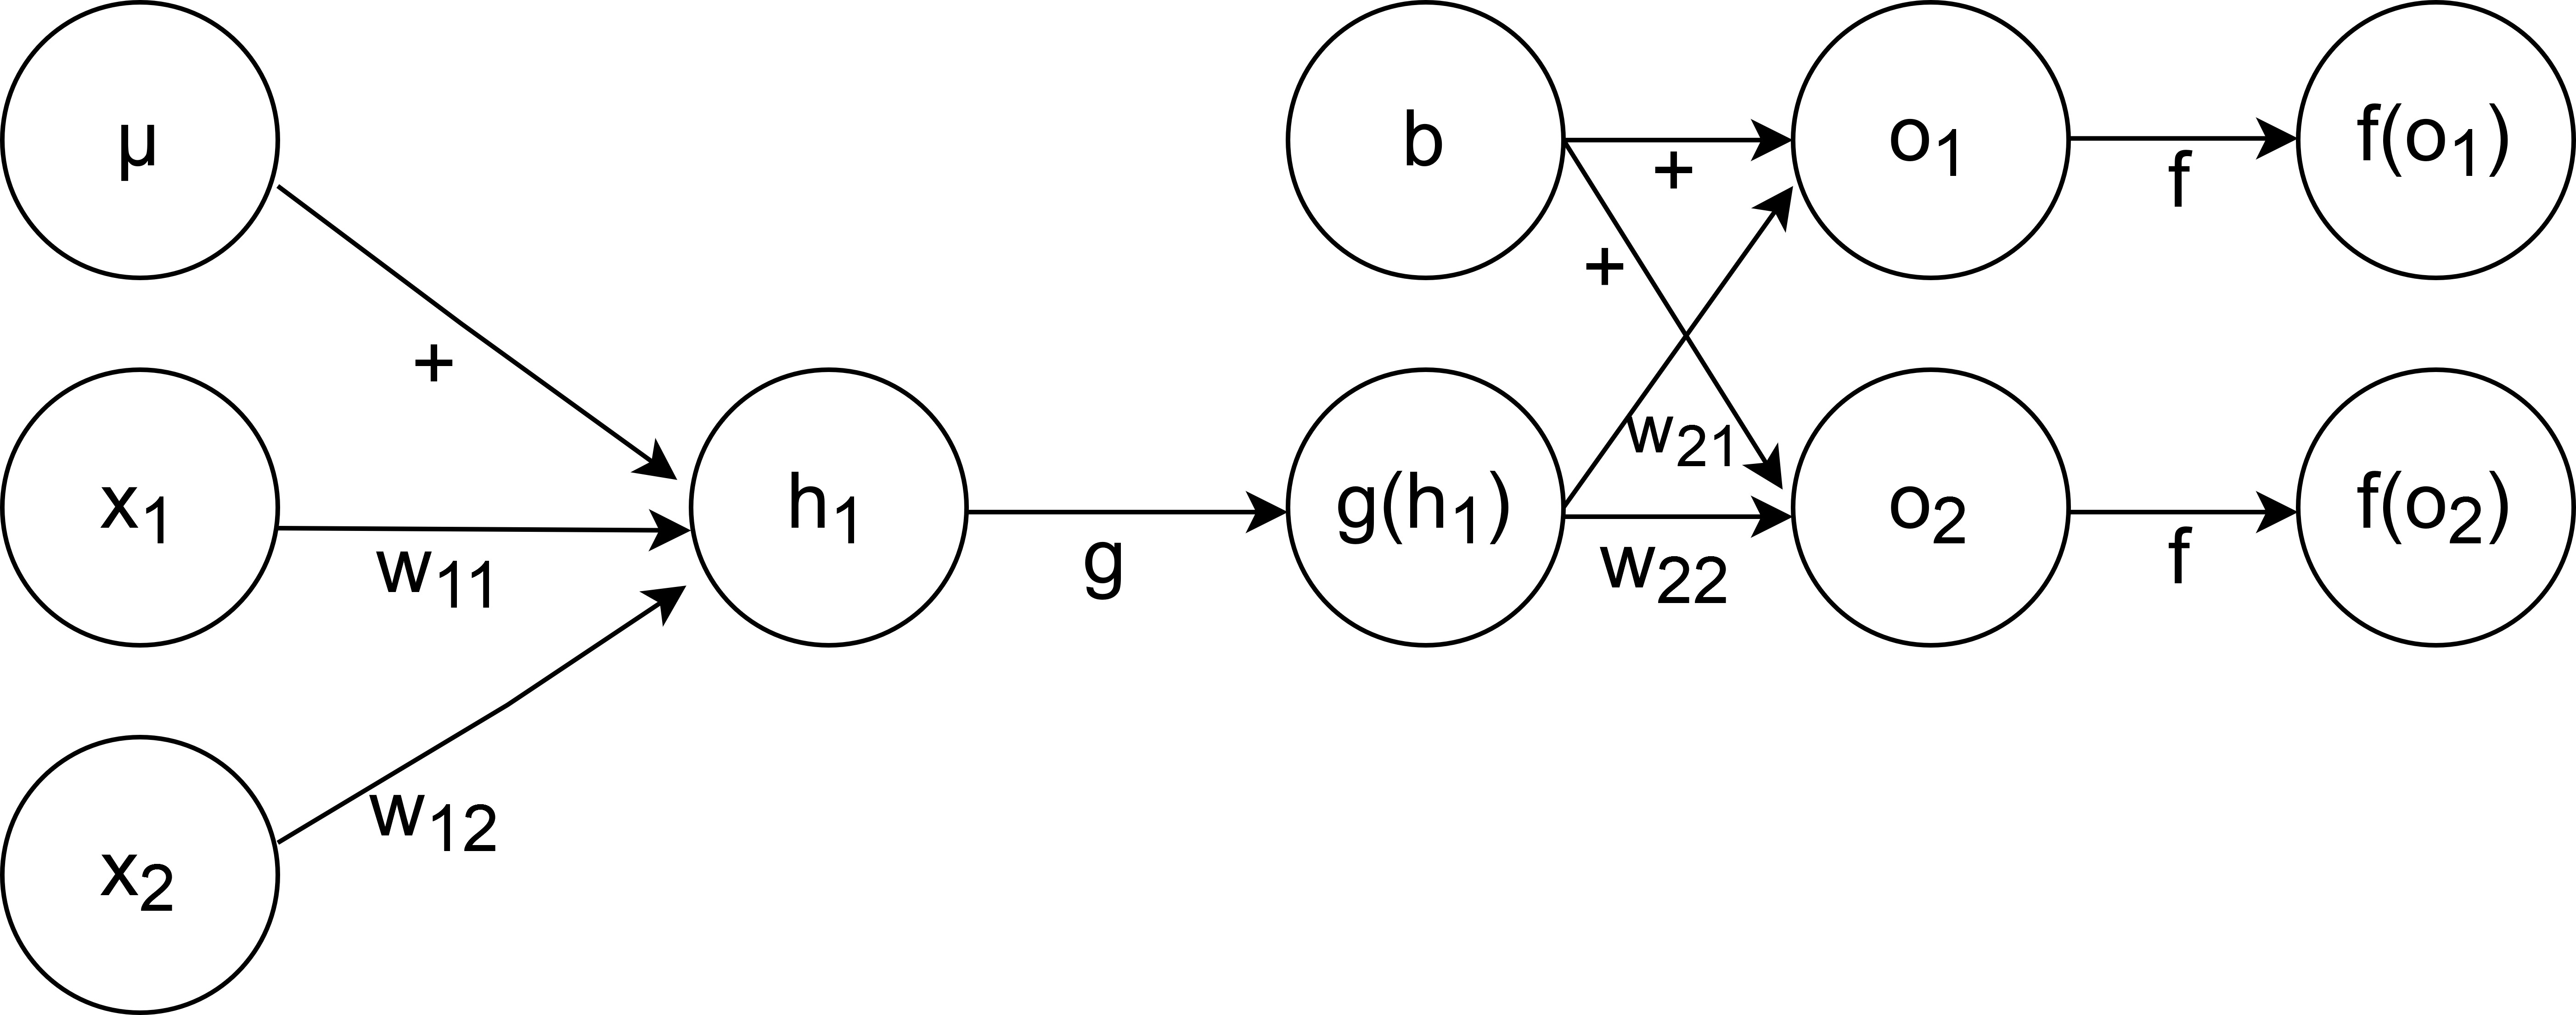
\includegraphics[width=1\textwidth]{images/computational_graph.jpg}
    \caption{Computational Graph of AutoRec instance with input dimension $d=2$ and hidden layer size $k=1$}
    \label{fig:autorec_example}
\end{figure}

\subsection{Naive Bayes \acrshort{cf}}
The Naive Bayes classifier is a model family that utilizes \texit{Bayes Theorem} combined with an independence assumption of the features to produce a classification. This model can be mapped to the \acrshort{cf} scenario \cite{valdiviezo2019collaborative}. \texit{Bayes Theorem} is defined as:\\
\begin{equation}
    P(A|B) = \frac{P(A)\cdot P(B|A)}{P(B)}
\end{equation}
In the above equation
\begin{itemize}
    \item $P(A)$ is called the \texit{prior probability}
    \item $P(B|A)$ is called the \texit{likelihood}.
    \item $P(B)$ is called the evidence.
    \item $P(A|B)$ is called the \texit{posterior probability}
\end{itemize}
Let there be $n$ different classes $c_1, c_2,\dots,c_n$ and $m$ features $f_1, f_2,\dots,f_m$.
In the case of the given data set there are two different classes $\{0,1\}$ for the conviction task and
seven different classes $\{0,1,2,3,4,5,6\}$ for the weight task.\\
Given a data vector $\Vec{f} \in \mathbb{R}^{m}$, the goal is to find the class $c$ that maximizes the following expression:\\
\begin{equation}
    \begin{align*}
        c^{*} = \arg\max_{c} P(c|\Vec{f})\\
        = \arg\max_{c} \frac{P(\Vec{f}|c)\cdot P(c)}{P(\Vec{f)}}\\
        \propto \arg\max_{c} P(\Vec{f}|c)\cdot P(c) \label{eq:1}  
    \end{align*}
\end{equation}
As the denominator in the above equation is independent on the class label $c$ for which the value needs to be found that maximizes the expression above, the equation is rewritten in form of a constant of proportionality.\\
Without the independence assumption the likelihood $P(\Vec{f}|c)$ would yield $m!$ factors.
With the independence assumption the joint probability can be written as the product of the single probabilities:
\begin{equation}
    \begin{align*}
        P(\Vec{f}|c) = P(f_1, f_2,\dots, f_m|c)\\
        = P(f_1|c)\cdot P(f_2|c) \dots P(f_m|c)
    \end{align*}
\end{equation}
The parts of the last expression of equation \eqref{eq:1} can be translated into the \acrshort{cf} scenario as follows:
\begin{equation}
    \begin{align*}
        \arg\max_{c} P(\Vec{f}|c)\cdot P(c) \;\widehat{=}\; \arg\max_{c} \prod\limits_{k \in I_u} P(r_{u_k}|r_{u_j}=c) \cdot P(r_{u_j} = c)
    \end{align*}
\end{equation}
The prior probability $P(r_{u_j} = c)$ is computed as the fraction of users who have specified the rating $c$ for item $j$ to all users that have specified any rating for item $j$.\\
The likelihood $\prod\limits_{k \in I_u} P(r_{u_k}|r_{u_j}=c)$ is based on the conditional independence assumption of the ratings.%Refactor this freaking sentence 
It is computed as the product of the fractions of users who have specified the rating $r_u_k$ for item $k$, given that they specified the rating for the $j$th item to $c$ to all users that have specified the rating for the $j$th item to c and have given a rating $c_k$ to item $k$ that is different from $r_{u_k}$ for every item $k \in I_u$. $I_u$ is the set of items the user $u$ has specified any rating for.\\
The final prediction will thus be:
\begin{equation}
    \begin{align*}
        \hat{r}_{u_j} = \arg\max_{c} \prod\limits_{k \in I_u} P(r_{u_k}|r_{u_j}=c) \cdot P(r_{u_j} = c)
    \end{align*}
\end{equation}

\subsection{User - Based Neighborhood Models}
The essence of user - based neighborhood models is to predict a rating for the target user - item pair $(u,i)$ based on a weighted rating of the $k$ most similar users $\tilde{u}_1, \dots ,\tilde{u}_k$ to the target user $u$ which made a prediction for item $i$. \\ 
A general issue in user - based neighborhood models is the fact that different users differ in their scale of ratings due to rating - biases \cite{wherry1982control}. Some users in general might give higher ratings whereas other users tend to give lower ratings. Approaches to tackle this problem will be proposed in the following.\\
Some definitions that are important for all the following user - based neighborhood models before proceeding are presented now.
$I_u$ denotes the set of items rated by user $u$. Given a rating matrix $R \in \mathbb{R}^{m \times n}$ with $m$ users and $n$ items, $r_u_j$ denotes the rating of user $u$ for item $j$. $\mathbbm{1_{u_j}}$ indicates if user $u$ has rated item $j$ or not. The average rating of user $u$ is defined as folows:
    \begin{equation}
    \mu_u = \frac{\sum\limits_{i \in I_u}r_u_i}{|I_u|}
    \end{equation}
In the following, different user - based neighborhood models will be presented.

\subsubsection{Mean - Centered Pearson Correlation}
The similarity of two users $u_1$ and $u_2$ is computed exclusively on the mutual observed ratings defined as $I_u_1 \cap I_u_2$.\\
The training - data sets that are provided specify $4$ ratings ($2$ for \acrshort{poc}, $2$ for \acrshort{pow}) for users for which predictions need to be made in the test - data set. So in general for these users of interest $U$ it holds that $|I_u| = 4\: \forall{u \in U}$.\\
A measure that can be applied to compute the similarity of two users $u_1, u_2$ is the \textit{Pearson Correlation Coefficient} \cite{benesty2009pearson}:
\begin{equation}
    \text{Pearson}(u_1, u_2) = \frac{\sum\limits_{i \in I_u_1 \cap I_u_2} (r_{u_1_i} - \mu_u_1) \cdot (r_{u_2_i} - \mu_u_2)}{\sqrt{\sum\limits_{i \in I_u_1 \cap I_u_2} (r_{u_1_i} - \mu_u_1)^2 \cdot \sum\limits_{i \in I_u_1 \cap I_u_2} (r_{u_2_i} - \mu_u_2)^2}}
\end{equation}
The Pearson Correlation Coefficient is computed for all user - pairs. Intuitively, the next step is to find the set $S$ of the $k$ users with the highest Pearson Correlation Coefficient to the target user to calculate a prediction.\\
As $R$ is sparse the number of mutually rated items by the users $u_1,\dots,u_k \in S$ is likely to change over different items. Therefore different sets of $S$ will be calculated for different items for the target user. It is also likely to happen that $|I_{u_1} \cap I_{u_2} \cap \dots \cap I_{u_k}| < I_{u_t}$ with $I_{u_t}$ being the target user and $u_1,\dots,u_k \in S$. In this case, the reduced number of neighbors will be used w.r.t. a similarity threshold $t$ that ensures that only ratings of users $u$ are considered in the prediction for which holds that $Pearson(u, u_t) >= t$.\\
The weighted average of these ratings will be used as the prediction for a specific item. The ratings will be weighted by the Pearson Correlation Coefficient of the owner to the target user.
Before actually producing predictions the problem of rating bias has to be tackled. To deal with rating biases the raw rating data is mean centered for every user:

\begin{equation}
    c_{u_j} = r_{u_j} - \mu_u
\end{equation}
Using the mean centered rating data, we can produce mean centered predictions for user item pairs $(u,j)$. To account for the centering, we add the mean $\mu_u$ of a specific user $u$ back to the prediction to produce a \textit{raw prediction}. Let $P_u(j,t)$ be the set of k - closest users to target user $u$ that specified a rating for item $j$ and for which $Pearson(u, v) >= t\;: \forall{v} \in P_u(j)$ holds.\\ The prediction function is defined as: 
\begin{equation}
    \hat{r}_{u_j} = \mu_u + \frac{\sum\limits_{v \in P_u(j)}\text{Pearson}(u, v) \cdot c_{v_j}}{\sum\limits_{v \in P_u(j)} |\text{Pearson}(u, v)|}
\end{equation}

\subsubsection{Significance Weighting}

The quality of the output of the similarity function for two users $u_i , u_j$ is related to the number of mutual rated items $|I_u \cap I_v|$. In general the assumption is made that more mutual rated items improve the similarity computation.\\
To account for this assumption the similarity function gets an additional parameter $\beta$. This parameter is a threshold for the number of mutual rated items $|I_u \cap I_v|$. The idea is to give the full weight to a calculated similarity value if $|I_u \cap I_v| >= \beta$ and reduce the weight if $|I_u \cap I_v| < \beta$. The weight should only take values from the interval $[0, 1]$. Given a calculated similarity value $Sim(u,v)$, the weighted similarity value $WeightedSim(u,v)$ is defined as:
\begin{equation}
    \text{WeightedSim}(u,v) = \text{Sim}(u,v) \cdot \frac{\min(|I_u \cap I_v|, \beta)}{\beta}, \;\beta \in \mathbb{N}
\end{equation}

\subsection{A Note on Item - Based Neighborhood Models}
In Item - Based Neighborhood Models the predictions of a target user - item pair $(u, i)$ is based on the weighted average of the $k$ most similar items $i_1,\dots,i_k$ the user $u$ has provided a rating for. As described in \ref{sec:difficulty}, only two items per task have a rating for the users in the training set for which a prediction needs to be made in the test set.\\
Therefore it is not feasible to apply an Item - Based Neighborhood Model in this scenario as there would only be two other ratings for which the corresponding items don't necessarily need to be similar.

\section{Results \& Discussion}
In the following the performance of the proposed models on all data set -/task - combinations using each of the discussed metrics will be discussed. This will be done in \autoref{chap:eval}. In \autoref{chap:efficiency} the computational efficiency of the proposed models will be discussed. The discussion of the hyperparameters is presented in \autoref{chap:hyperparams}.

\subsection{Evaluation}
\label{chap:eval}
In the following the margins of performance differences are computed as the difference between the best baseline performance and the best non - baseline performance.\\ 

\noindent In Table \ref{tab:results} the performance results of the models using the provided metrics accuracy (\acrshort{poc}) and \acrshort{rmse} (\acrshort{pow}) are presented. It can be observed that for the tasks defined on $T_1 \to T_2$ the \acrfull{nn} - classifier achieves the best performance by a margin of 0.1\% (\acrshort{poc}) and 29.4\% (\acrshort{pow}). For the tasks defined on $T_2 \to T_3$ the \acrshort{iautorec} model achieves the best performance by a margin of 6.8\% (\acrshort{poc}) and 19.8\% (\acrshort{pow}) compared to the best baseline model. As discussed in \ref{chap:subdivison} accuracy as well as \acrshort{rmse} are not reasonable metrics to use on this data set as the distribution of ratings within single items is highly skewed.

\begin{table}[h!]
    \centering
    \begin{tabular}{|c|c|c|c|c|}
    \hline
     & \multicolumn{2}{|c|}{\acrshort{poc} (Accuracy)} & \multicolumn{2}{|c|}{\acrshort{pow} (\acrshort{rmse})} \\
     \hline
    Algorithms & $T_1 \to T_2$ & $T_2 \to T_3$ & $T_1 \to T_2$ & $T_2 \to T_3$\\
    \hline  Majority (baseline) & \textbf{.783} & .737 & 3.26 & 3.52 \\
    \acrshort{nn} (baseline) & \textbf{.783} & .738 & \textbf{2.86} & 2.53\\
    \acrshort{tlmf} & .782 & .788 & 3.70 & 2.40 \\
    \acrshort{tlmf} + Bert & .780 & .785 & 3.70 & 2.41\\
    Naive Bayes & .782 & .802 & 5.96 & 2.99 \\
    I - AutoRec & .730 & \textbf{.806} & 4.13 & \textbf{2.03}\\
    User - Neighborhood (Pearson) & .593 & .617 & 7.53 & 4.71\\
    \hline
    \end{tabular}
    \caption{Results of the Models, Evaluated With the Provided Metrics.}
    \label{tab:results}
\end{table}
\noindent In Table \ref{tab:results_f1_mean} the performance results of the models using the averaged F - score are presented. It can be seen that the \acrshort{tlmf} model performs best on the \acrshort{poc} task for the $T_1 \to T_2$ data set by a margin of 3.2\%. For the respective \acrshort{pow} task the Naive Bayes model performs best by a margin of 15\%. Likewise, the Naive Bayes model shows the best performance for tasks defined on $T_2 \to T_3$. It achieves the best performance by a margin of 7.8\% (\acrshort{poc}) and 43.4\%, respectively.

\begin{table}[h!]
    \centering
    \begin{tabular}{|c|c|c|c|c|}
    \hline
     & \multicolumn{2}{|c|}{\acrshort{poc} (F1 - Score)} & \multicolumn{2}{|c|}{\acrshort{pow} (F1 - Score)} \\
     \hline
    Algorithms & $T_1 \to T_2$ & $T_2 \to T_3$ & $T_1 \to T_2$ & $T_2 \to T_3$\\
    \hline  Majority (baseline) & .411 & .387 & .115 & .108 \\ 
    \acrshort{nn} (baseline) & .746 & .720 & .080 & .104\\
    \acrshort{tlmf} & \textbf{.778} & .784 & .191 & .481\\
    \acrshort{tlmf} + Bert & .777 & .780  & .191 & .481 \\
    Naive Bayes & .770 & \textbf{.798} & \textbf{.265} & \textbf{.561} \\
    I - AutoRec & .722 & .784 & .202 & .542\\
    User - Neighborhood (Pearson) & .542 & .602 & .188 & .108\\
    \hline
    \end{tabular}
    \caption{Results of the Models, Evaluated With the Average F1 – Score.}
    \label{tab:results_f1_mean}
\end{table}
\noindent In Table \ref{tab:results_precision_mean} the performance results of the models using the averaged precision score are presented. For data set $T_1 \to T_2$ the \acrshort{tlmf} model and the Naive Bayes model achieve the highest performance by a margin of 2.9\% (\acrshort{poc}) and 7.7\%, respectively. For data set $T_2 \to T_3$ the Naive Bayes model and the \acrshort{iautorec} model achieve the highest performance by a margin of 18.1\% and 48\%, respectively.
\begin{table}[h!]
    \centering
    \begin{tabular}{|c|c|c|c|c|}
    \hline
     & \multicolumn{2}{|c|}{\acrshort{poc} (Precision)} & \multicolumn{2}{|c|}{\acrshort{pow} (Precision)} \\
     \hline
    Algorithms & $T_1 \to T_2$ & $T_2 \to T_3$ & $T_1 \to T_2$ & $T_2 \to T_3$\\
    \hline  Majority (baseline) & .404 & .367 & .099 & .085 \\ 
    \acrshort{nn} (baseline) & .759 & .725 & .085 & .103\\
    \acrshort{tlmf} & \textbf{.788} & .778 & .236 & .531 \\
    \acrshort{tlmf} + Bert & .787 & .774 & .236 & .481\\
    Naive Bayes & .775 & \textbf{.802} & \textbf{.266} & .574 \\
    I - AutoRec & .731 & .783 & .260 & \textbf{.583}\\
    User - Neighborhood (Pearson) & .558 & .612 & .181 & .181\\
    \hline
    \end{tabular}
    \caption{Results of the Models, Evaluated With the Average Precision – Score.}
    \label{tab:results_precision_mean}
\end{table}\\
\noindent In Table \ref{tab:results_recall_mean} the performance results of the models using the averaged recall score are presented. For data set $T_1 \to T_2$ the \acrshort{tlmf} model performs best by a margin of 3.6\% (\acrshort{poc}) and 8.1\% (\acrshort{pow}). For data set $T_2 \to T_3$ the naive bayes model performs best by a margin of 6.6\% (\acrshort{poc}) and 40.9\% (\acrshort{pow}).

\begin{table}[h!]
    \centering
    \begin{tabular}{|c|c|c|c|c|}
    \hline
     & \multicolumn{2}{|c|}{\acrshort{poc} (Recall)} & \multicolumn{2}{|c|}{\acrshort{pow} (Recall)} \\
     \hline
    Algorithms & $T_1 \to T_2$ & $T_2 \to T_3$ & $T_1 \to T_2$ & $T_2 \to T_3$\\
    \hline  Majority (baseline) & .419 & .410 & .202 & .178 \\ 
    \acrshort{nn} (baseline) & .741 & .718 & .145 & .147\\
    \acrshort{tlmf} & \textbf{.777} & \textbf{.799} & .223 & .497 \\
    \acrshort{tlmf} + Bert & .776 & \textbf{.799} & .223 & .497\\
    Naive Bayes & .763 & .796 & \textbf{.268} & \textbf{.556} \\
    I - AutoRec & .714 & .786 & .223 & .552\\
    User - Neighborhood (Pearson) & .550 & .604 & .224 & .153\\
    \hline
    \end{tabular}
    \caption{Results of the Models, Evaluated With the Average Recall – Score.}
    \label{tab:results_recall_mean}
\end{table}\\

\noindent In Table \ref{tab:results_g_mean} the performance results of the models using the averaged G - mean are presented. For data set $T_1 \to T_2$ the \acrshort{tlmf} model achieves the best performance with by a margin of 4.1\% (\acrshort{poc}) and 8.3\% (\acrshort{pow}). For data set $T_2 \to T_3$ the naive bayes model performs best by a margin of 16.4\% (\acrshort{poc}) and 44.7\%. 

\begin{table}[h!]
    \centering
    \begin{tabular}{|c|c|c|c|c|}
    \hline
     & \multicolumn{2}{|c|}{\acrshort{poc} (G - Mean)} & \multicolumn{2}{|c|}{\acrshort{pow} (G - Mean)} \\
     \hline
    Algorithms & $T_1 \to T_2$ & $T_2 \to T_3$ & $T_1 \to T_2$ & $T_2 \to T_3$\\
    \hline  Majority (baseline) & .300 & .299 & .299 & .270 \\ 
    \acrshort{nn} (baseline) & .731 & .714 & .255 & .285\\
    \acrshort{tlmf} & \textbf{.772} & \textbf{.797} & .408 & .672 \\
    \acrshort{tlmf} + Bert & .771 & .796 & .408 & .672\\
    Naive Bayes & .758 & .794 & \textbf{.463} & \textbf{.717} \\
    \acrshort{iautorec} - AutoRec & .724 & .786 & .431 & .715\\
    User - Neighborhood (Pearson) & .501 & .590 & .342 & .270\\
    \hline
    \end{tabular}
    \caption{Results of the Models, Evaluated With the Average G - Mean.}
    \label{tab:results_g_mean}
\end{table}
\noindent It can be observed that the Naive Bayes model as well as the \acrshort{tlmf} model perform remarkably well. The Naive Bayes model achieves the best performance in 62.5\% cases of all task / data set combinations for the newly introduced metrics. The \acrshort{tlmf} model achieves the best performance in 31.25\% of the cases. It can also be seen that the User Neighborhood model is performing significantly worse than the other proposed models. This is likely caused by the fact that too little rating data is available for most users to compute reasonable user - similarity clusters.
It can also be observed that the argument - similarity matrix computed by the \acrshort{bert} model does not seem to enhance the prediction power of the matrix factorization model in comparison to the similarity matrix computed by the less complex \acrshort{wtmf} model.\\
As predicted, the baseline models are far off from the best performance in every evaluation instance. This supports the assumption that the choice of accuracy and \acrshort{rmse} as the evaluation metrics is not suitable for the data set at hand.\\
In general, the performance difference of the baseline models and the proposed models is greater for the data set $T_2 \to T_3$. One explanation could be the fact that $T_2 \to T_3$ is less sparse and more balanced than $T1 \to T_2$. This can be observed from Table \ref{tab:my_label}.\\
Overall the models perform generally worse in the \acrshort{poc} task than in the \acrshort{pow} task on the same data sets. This is likely due to the fact that the \acrshort{pow} task is more complex.

\subsection{Computational Efficiency}
\label{chap:efficiency}
\subsubsection{\acrshort{tlmf}}
The largest share of the computation costs can be attributed to the creation of the argument embeddings in the first step of the \acrshort{tlmf} \cite{li2016two}. This involves optimizing the objective function by calculating the gradients and updating the corresponding vectors in the latent - factor matrices. The computational cost of the first level of the \acrshort{tlmf} for optimizing the objective function can therefore be stated as $O(N a K)$ with $N$ being the number of sentenes in the corpus, $K$ being the embedding dimension and $a$ being the average number of words per argument. The computational cost to update the corresponding word vectors is given by $O(M a K)$ where M is the number of words in the textual corpus. Similarly, the computational cost to update the corresponding sentence vectors is given by $O(N a K)$. Thus, the optimization of the lower level matrix factorization is highly dependent on the length of the sentences $N$ as well as the embedding dimension $K$.\\
The computational cost for the second step consists of optimizing the objective function ($O(m\Bar{r}d + m\Bar{t}d)$) where $m$ is the number of items, $d$ is the embedding dimension,
$\Bar{r}$ is the average number of ratings per item and $\Bar{t}$ is the average number of ratings of the most similar neighbors per item. The cost of evaluating the corresponding user vectors is $O(n\Bar{x}d)$ with $n$ being the number of users and $\Bar{x}$ being the average number of ratings per user. Similarly the computational cost of evaluating the corresponding item vectors is $O(m\Bar{x}d + m\Bar{t}d)$.\\ Therefore the computation of the objective function as well as the computation of the corresponding vectors are linear with respect to the number of users and items in the data set. The cost of a prediction is $O(d + d) = O(d)$ as a $d$ dimensional dot - product needs to be computed with $d$ multiplications and $d$ additions.

\subsubsection{\acrshort{iautorec}}
In the following the dimension of the input layer will be denoted with $n$, the dimension of the hidden layer will be denoted with $h$ and the dimension of the output layer will be denoted with $m$.\\
A perceptron in the hidden layer with $n$ inputs will perform $n + 1$ multiplications (dot - product and bias terms) and $n + 1$ additions (dot - product and bias term). Afterwards one operation has to be done to evaluate the activation function.\\
The computational complexity of one perceptron in the hidden state can be approximated by\\
\begin{equation}
    O((n+1) + (n+1) + 1) = O(n)
\end{equation} 
As this needs to be done by all perceptrons in the hidden layer, the total computational complexity of the hidden layer can be stated as $h \cdot O(n)$. The same procedure is repeated for the output layer. The output layer gets $h$ inputs. Thus, a $h + 1$ dimensional dot product needs to be computed with a succeeding operation for the activation function. Its' computational complexity can be stated as\\
\begin{equation}
    O((h +1) + (h + 1) + 1 = O(h)
\end{equation}
Scaled by the number of perceptrons in the output layer, the computational complexity of the output layer can be described as\\
\begin{equation}
    m \cdot O(h)
\end{equation}
Thus, the computational complexity of a forward pass, i.e. the computational cost of making a prediction, is given by\\
\begin{equation}
    m \cdot O(h) + h \cdot O(n) = O((n + m) \cdot h)
\end{equation}
Doing a forward pass with succeeding backpropagation of the error to adjust the weights changes the computational complexity to\\
\begin{equation}
    2 \cdot O((n + m) \cdot h) = O((n + m) \cdot h)
\end{equation}
The computational complexity for training the \acrshort{iautorec} model is therefore\\
\begin{equation}
    k \cdot e \cdot O((n + m) \cdot h)
\end{equation}
where $e$ is the number of epochs the model trains and $k$ is the number of samples in the training set.

\subsubsection{Naive Bayes \acrshort{cf}}
The computational cost for computing the prior - probability is given by\\
\begin{equation}
    O(I \cdot C)
\end{equation}
where I is the number of items and C is the number of classes.
The computational cost for computing the users that rated a specific item with a specific class is given by\\
\begin{equation}
    O(\bar{I} \cdot \bar{U} \cdot C)
\end{equation}
where $\bar{I}$ is the average number of ratings for an argument and $\bar{U}$ is the average number of ratings given by a user.\\
These two calculations are implemented in the training phase. That means the computational complexity of the training phase is given by:\\
\begin{equation}
    O((I \cdot C) + (\bar{I} \cdot \bar{U} \cdot C))\\ = O(C \cdot (I + (\bar{I} \cdot \bar{U})
\end{equation}
That means that the training phase is linear in the size and sparsity of the training rating matrix as $C$ tends to be very small (typically $2 \leq C \leq 8$).\\
The likelihood is computed when making predictions, not in the training phase. Therefore the computational cost for making a prediction is given by:\\
\begin{equation}
    O((C \cdot \bar{I} \cdot \bar{U}))
\end{equation}
If the likelihood computation for all users and items is carried out in the training phase, the computational cost for making a prediction even reduces to $O(1)$ as two hashtable lookups with succeeding multiplication need to be executed. In this case, the term $(C \cdot I \cdot U)$ would be added to the computational cost of the training.

\subsubsection{User Neighborhood}
Normally, neighborhood models are divided into two phases: an offline phase and an online phase \cite{aggarwal2016recommender}. In the offline phase the similarity computation is carried out. In the online phase, a prediction is made using the previously calculated similarity values.
Let $u$ denote the maximal number of specified ratings of a user and let $i$ denote the maximal number of specified ratings of an item. Then the computational complexity for calculating the similarity value of one user to the other users in the offline phase is given by $O(u \cdot i)$. 
To determine the calculation time for all users, the previously mentioned expression is multiplied by the maximum number of specified ratings for an item, leading to the computational complexity of $O(i^2 \cdot u)$.\\
Regarding the online phase, the computational complexity of predicting a rating is given by $O(k)$ with $k$ being the user - neighborhood size that is used for prediction.
\subsection{Hyperparameters}
\label{chap:hyperparams}
The hyperparameters for the parameterizable models were chosen based on the best performance on the validation data set. It is important to note that for each model the same set of hyperparameter values are used for the different metrics.\\
It is noteworthy that the best performing Naive Bayes model does not need to be tuned as it does not contain any tuneable parameters.\\
It can be observed from Table \ref{tab:tlmf} and Table \ref{tab:autorec} that the embedding dimension that yields the best results for the \acrshort{tlmf} model and the \acrshort{iautorec} model is much smaller for the \acrshort{poc} task than for the \acrshort{pow} task, implying that the \acrshort{poc} task is less complex than the \acrshort{pow} task.\\ 
The hyperparameter values that were used to obtain the claimed performances are presented in \ref{chap:pvo}.

\subsection{Conclusion}
In this thesis, several recommendation algorithms were implemented and evaluated on metrics that took into account the class distribution of the rating data, such as G - Mean and F - Score.\\
The original evaluation metrics accuracy and rmse were not reasonable to use for assessing the performance of the proposed baseline algorithms as the class distribution within single items was imbalanced.\\
Evaluating on the proposed metrics showed that the baseline algorithms were outperformed on every task -/data set - combination. Especially the Naive Bayes algorithm and the \acrshort{tlmf} algorithm performed well with the Naive Bayes algorithm being the more efficient one of them without the need to tune this algorithm.
 
\clearpage
\section{Appendix}
\subsection{Parameter Values Overview}
\label{chap:pvo}
This section provides information about the parameter values that were used in the different models to obtain the claimed results and to reproduce them using the provided source code.

\begin{table}[h!]
    \centering
    \begin{tabular}{|c|c|}
        \hline Parameter & Value \\
        \hline  $k$ & 20 \\
        iterations & 30 \\
        $w$ & .01 \\
        $\gamma$ & .01 \\
        random - seed & 8 \\
    \hline    
    \end{tabular}
    \caption{Parameter Values Used in the WTMF, the First Step of the \acrshort{tlmf}.}
    \label{tab:wtmf}
\end{table}

\begin{table}[h!]
    \centering
    \begin{tabular}{|c|c|c|c|c|}
        \hline
         & \multicolumn{4}{|c|}{Values} \\
        \hline & \multicolumn{2}{|c|}{\acrshort{poc}} & \multicolumn{2}{|c|}{\acrshort{pow}} \\
        \hline Parameter & $T_1 \to T_2$  & $T_2 \to T_3$  & $T_1 \to T_2$  & $T_2 \to T_3$ \\
        \hline  $d$ & 1 & 3 & 20 & 20\\
          iterations & 17 & 23 & 201 & 201\\
          r & .041 & .001 & .1 & .1\\
          $\alpha$ & .0001 & .0009 & .0001 & .0001\\
          random - seed & 46 & 514 & 262 & 262\\
          $\eta$ & .031 & .081 & .005 & .005\\
          $n$ & 74 & 18 & 3 & 3\\
        \hline
    \end{tabular}
    \caption{Parameter Values Used in the \acrshort{tlmf} for the Different Task/Data Set Combinations.}
    \label{tab:tlmf}
\end{table}

\begin{table}[h!]
    \centering
    \begin{tabular}{|c|c|c|c|c|}
        \hline
         & \multicolumn{4}{|c|}{Values} \\
        \hline & \multicolumn{2}{|c|}{\acrshort{poc}} & \multicolumn{2}{|c|}{\acrshort{pow}} \\
        \hline Parameter & $T_1 \to T_2$  & $T_2 \to T_3$  & $T_1 \to T_2$  & $T_2 \to T_3$ \\
        \hline  $k$ & 6 & 90 & 200 & 200\\
          iterations & 358 & 29 & 200 & 200\\
          random - seed & 7 & 3 & 7 & 7\\
          $\eta$ & .001 & .001 & .0001 & .0001\\
        \hline
    \end{tabular}
    \caption{Parameter Values Used in the \acrshort{iautorec} Model for the Different Task/Data set Combinations.}
    \label{tab:autorec}
\end{table}

\begin{table}[h!]
    \centering
    \begin{tabular}{|c|c|c|c|c|}
        \hline
         & \multicolumn{4}{|c|}{Values} \\
        \hline & \multicolumn{2}{|c|}{\acrshort{poc}} & \multicolumn{2}{|c|}{\acrshort{pow}} \\
        \hline Parameter & $T_1 \to T_2$  & $T_2 \to T_3$  & $T_1 \to T_2$  & $T_2 \to T_3$ \\
        \hline  $k$ & 36 & 1 & 12 & 38\\
          similarity threshold & .87 & .7 & .4 & .63\\
        \hline
    \end{tabular}
    \caption{Parameter Values Used in the User Neighborhood Model for the Different Task/Data Set Combinations.}
    \label{tab:autorec}
\end{table}
\clearpage

\subsection{Plots}
\label{sec:plots}

\begin{figure}[!ht]
    \centering
    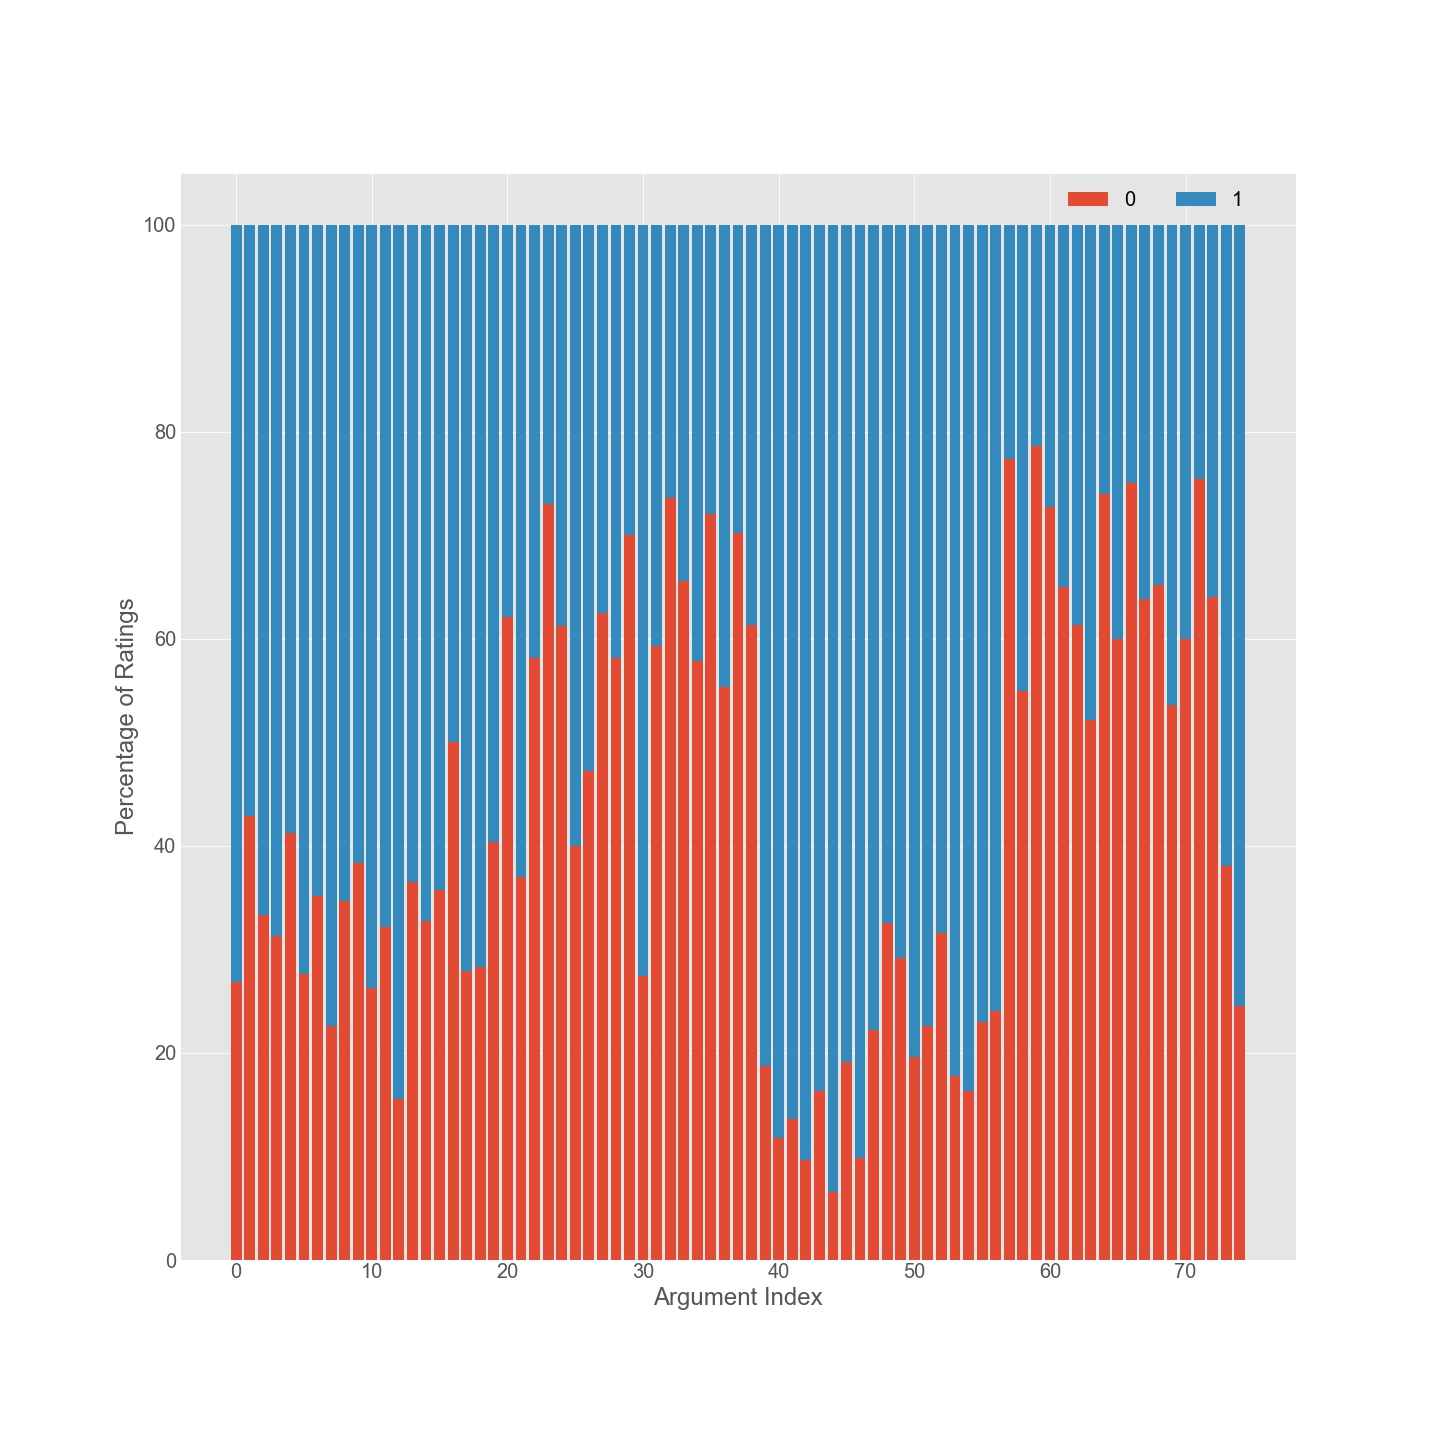
\includegraphics[width=1\textwidth]{images/T1_T2_train_Conviction.jpg}
    \caption{Distribution of the Train – Ratings Given for Arguments in $T_1 \to T_2$ in Percentage for the Conviction Task.}
    \label{fig:conviction_t1_t2_train}
\end{figure}

\begin{figure}[!ht]
    \centering
    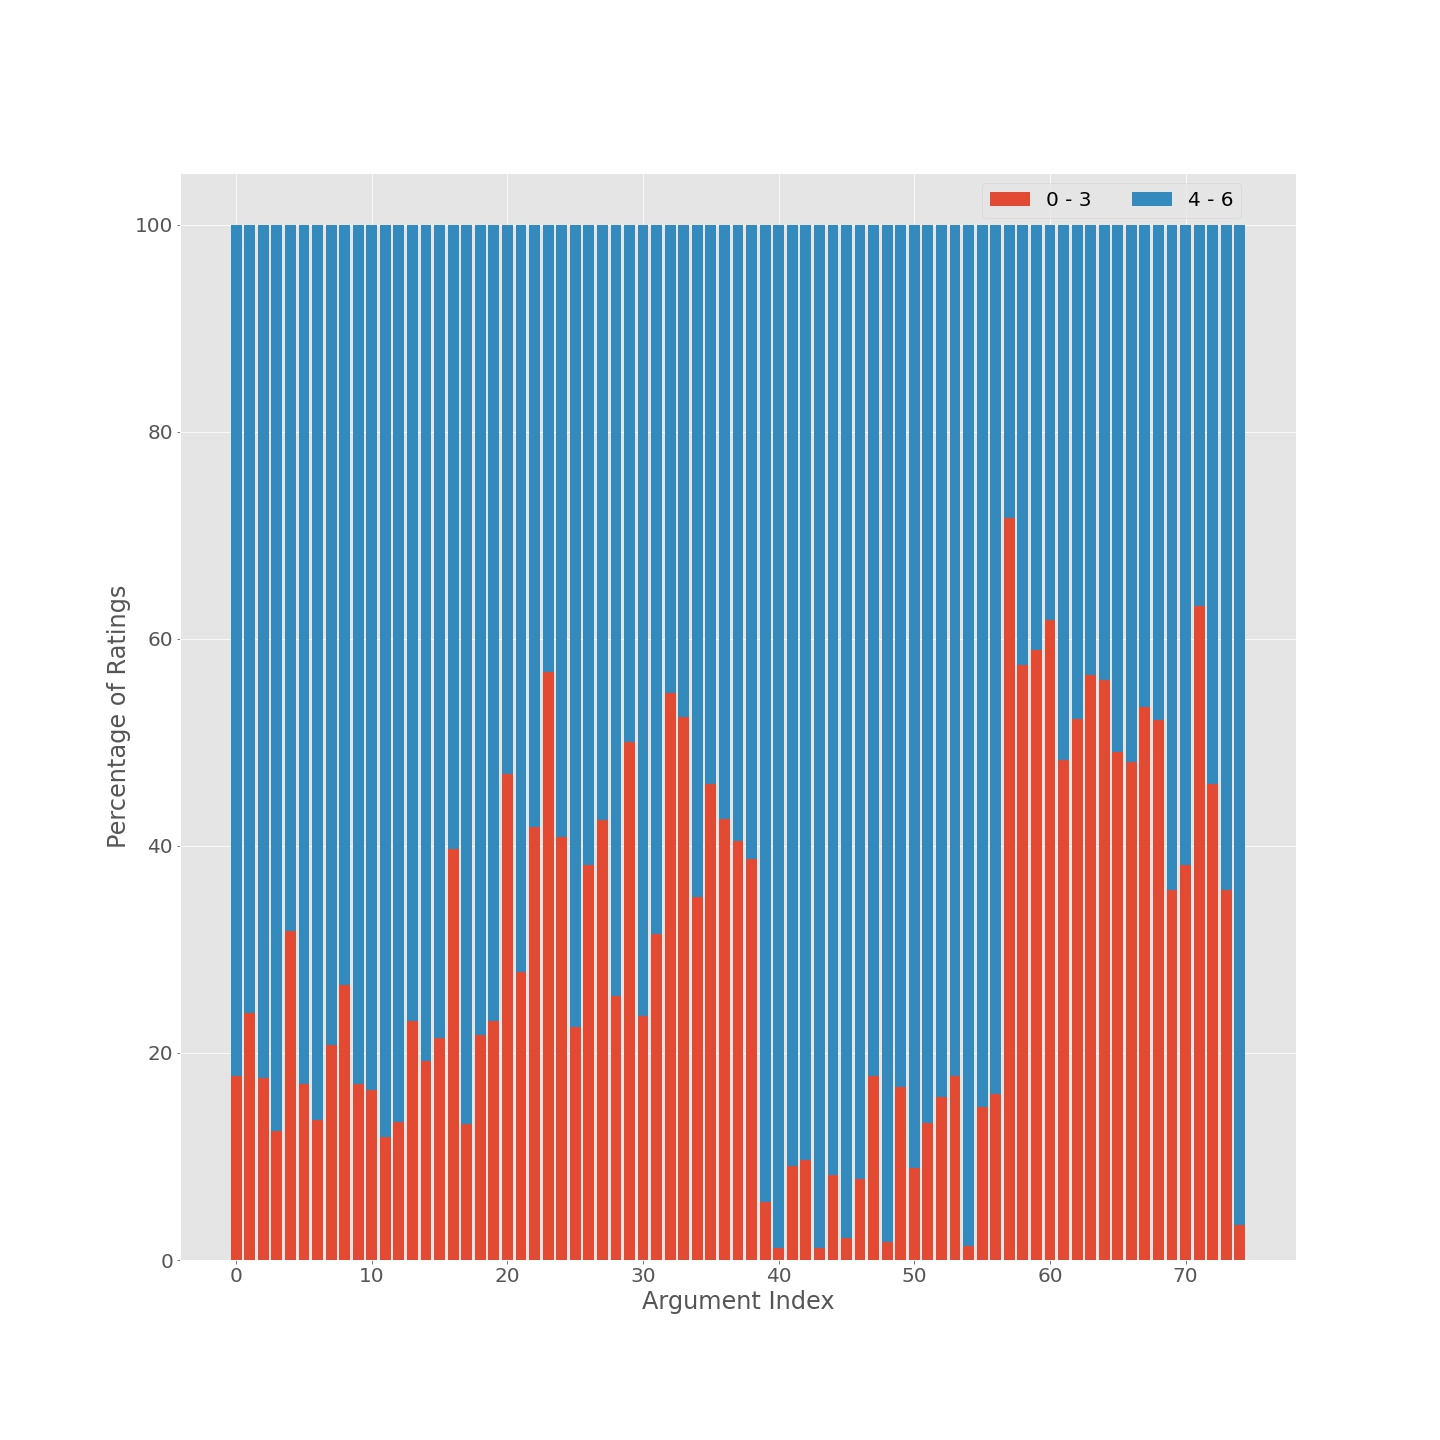
\includegraphics[width=1\textwidth]{images/T1_T2_train_Weight.jpg}
    \caption{Distribution of the Train – Ratings Given for Arguments in $T_1 \to T_2$ in Percentage for the Weight Task, Grouped by Rating Values 0 - 3 and 4 - 6.}
    \label{fig:conviction_t1_t2_train}
\end{figure}

\begin{figure}[!ht]
    \centering
    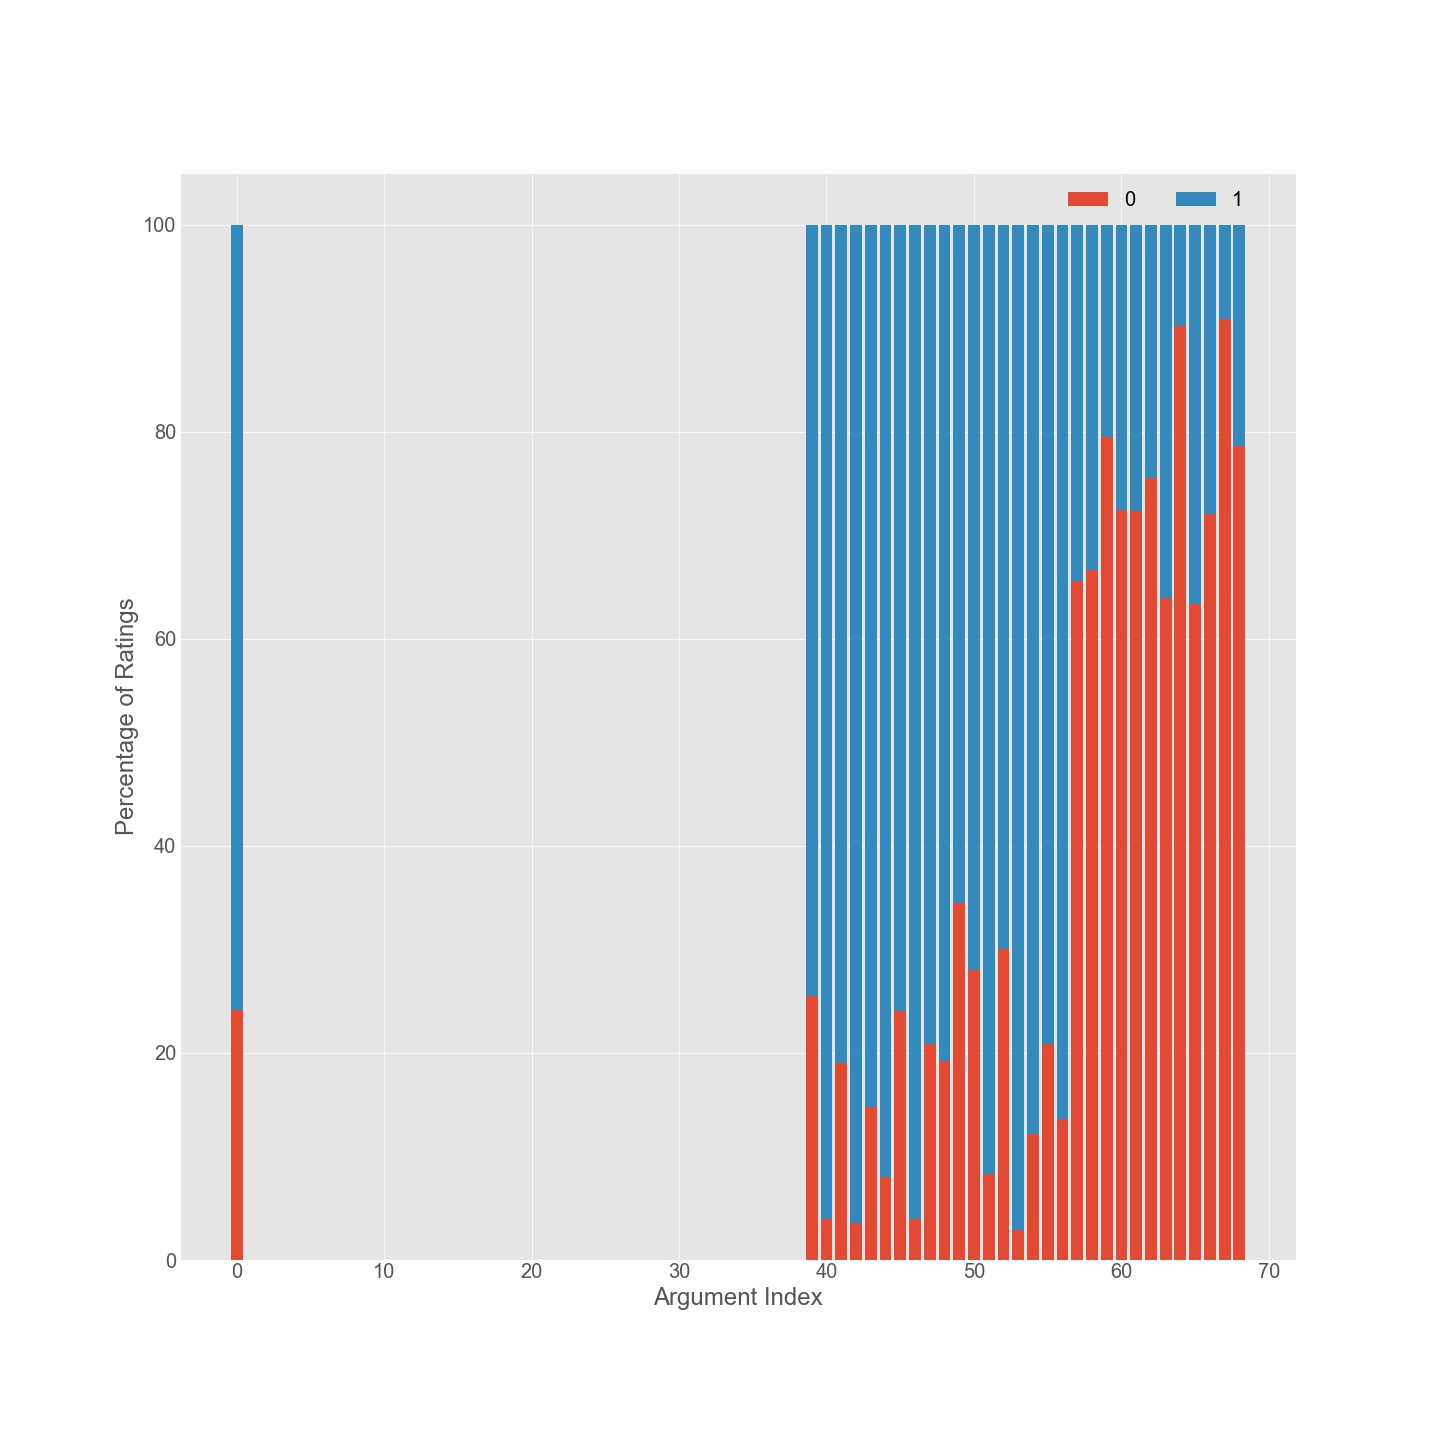
\includegraphics[width=1\textwidth]{images/T1_T2_test_Conviction.jpg}
    \caption{Distribution of the Test – Ratings Given for Arguments in $T_1 \to T_2$ in Percentage for the Conviction Task.}
    \label{fig:conviction_t1_t2_test}
\end{figure}

\begin{figure}[!ht]
    \centering
    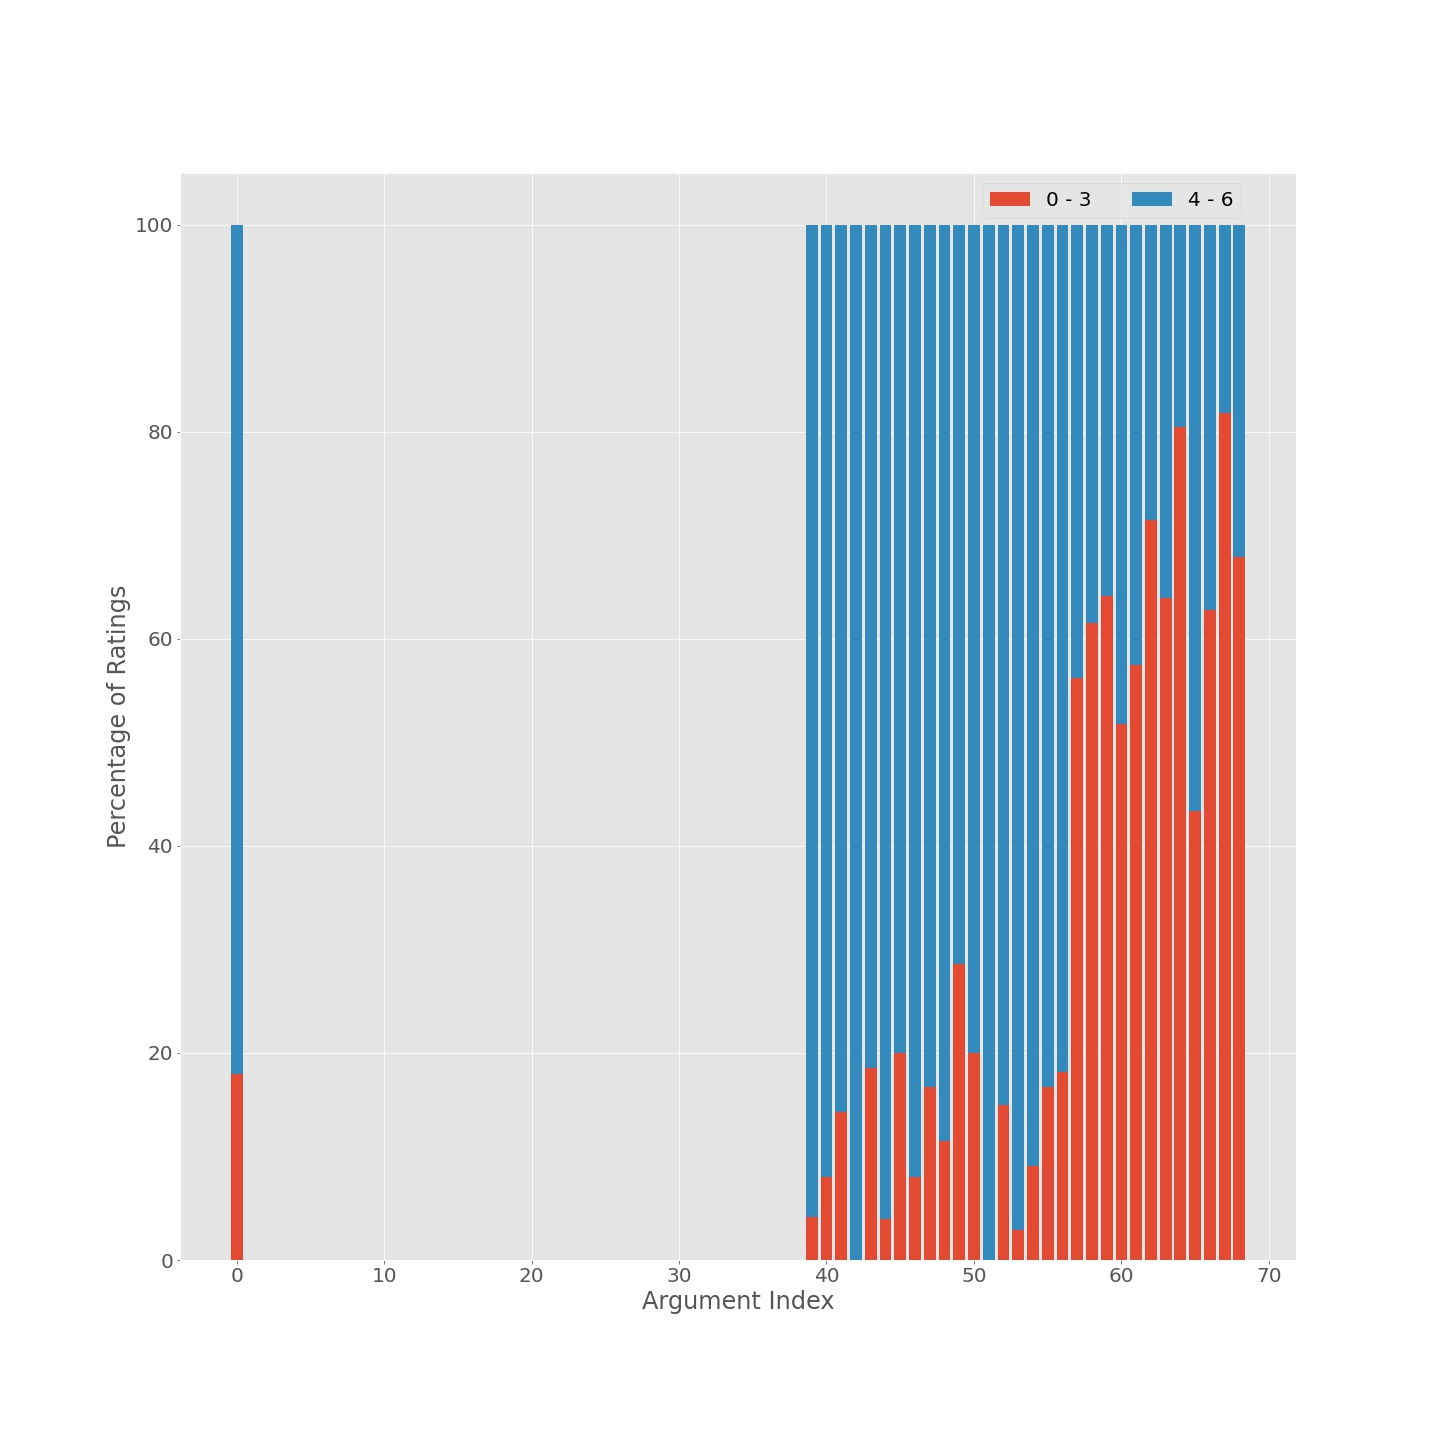
\includegraphics[width=1\textwidth]{images/T1_T2_test_Weight.jpg}
    \caption{Distribution of the Test – Ratings Given for Arguments in $T_1 \to T_2$ in Percentage for the Weight Task.}
    \label{fig:conviction_t2_t3_test}
\end{figure}

\begin{figure}[!ht]
    \centering
    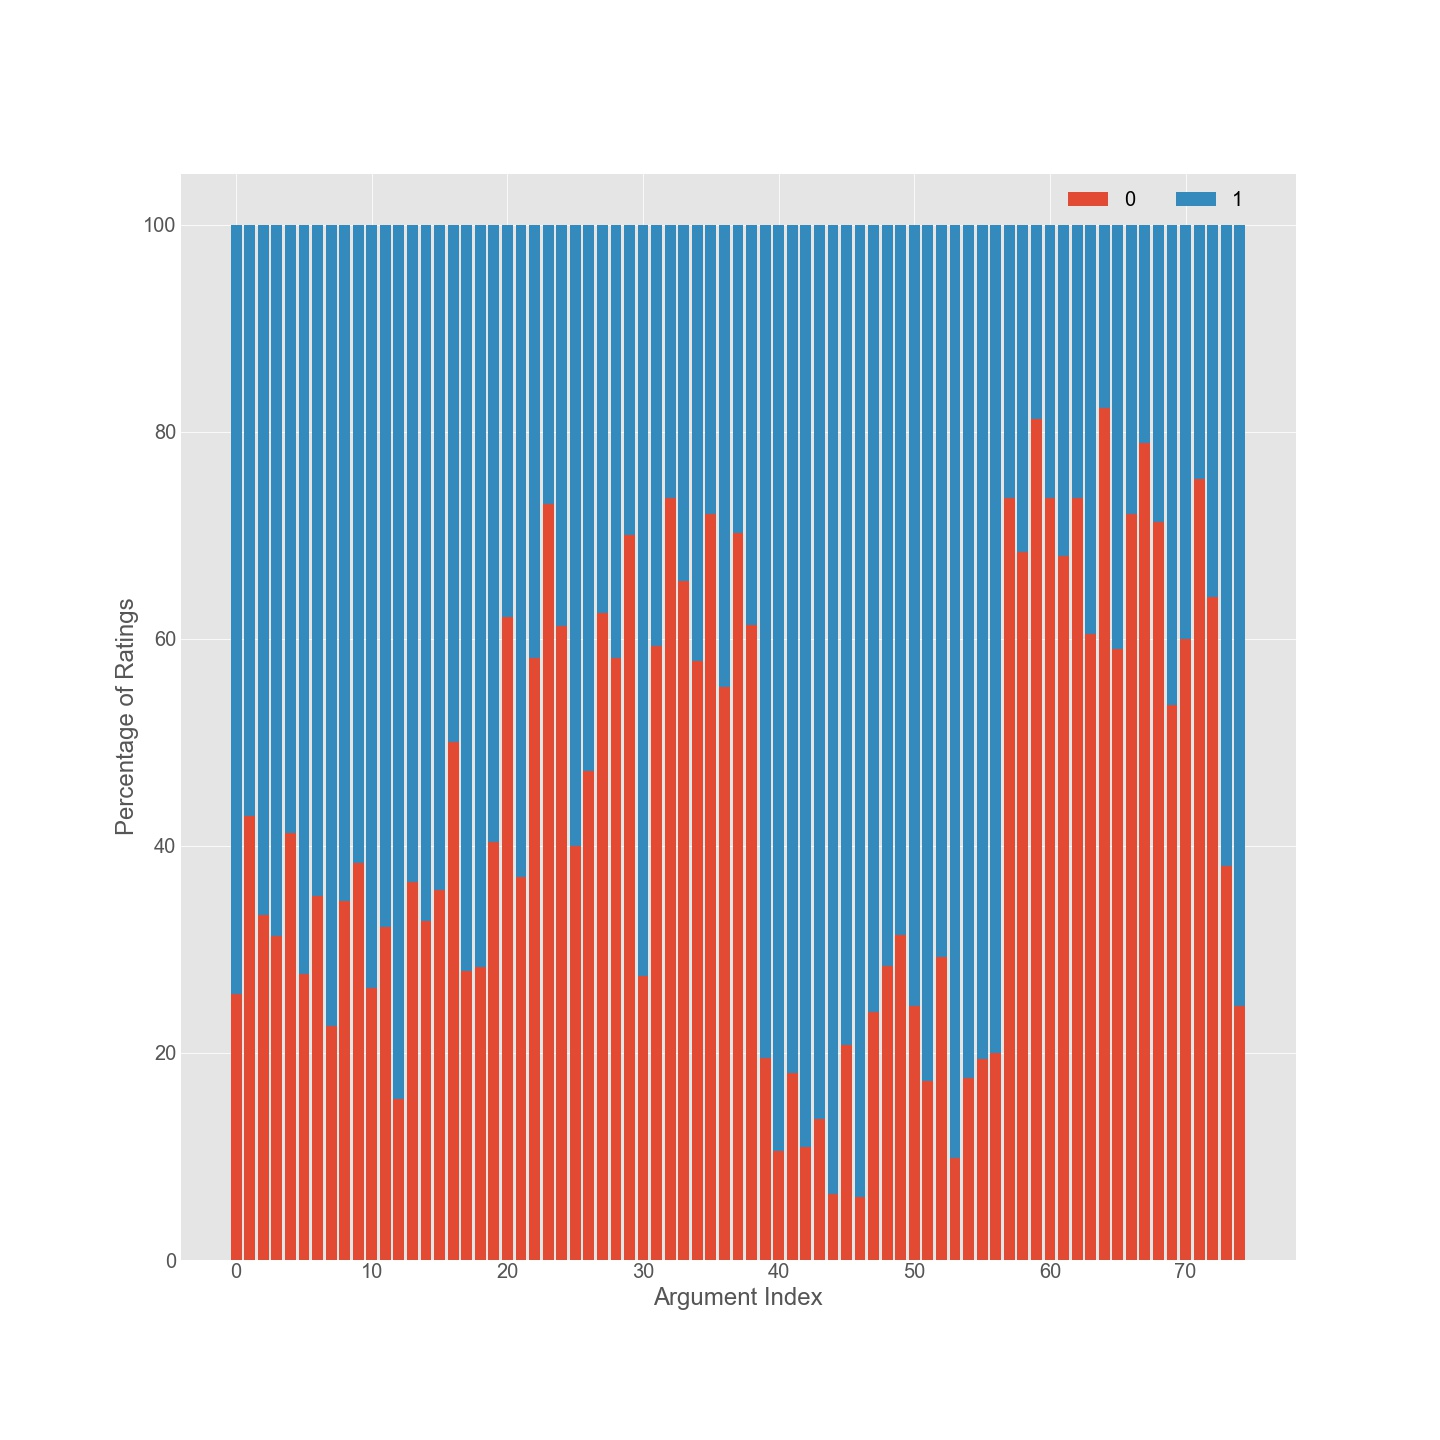
\includegraphics[width=1\textwidth]{images/T2_T3_train_Conviction.jpg}
    \caption{Distribution of the Train – Ratings Given for Arguments in $T_2 \to T_3$ in Percentage for the Conviction Task.}
    \label{fig:conviction_t2_t3_train}
\end{figure}

\begin{figure}[!ht]
    \centering
    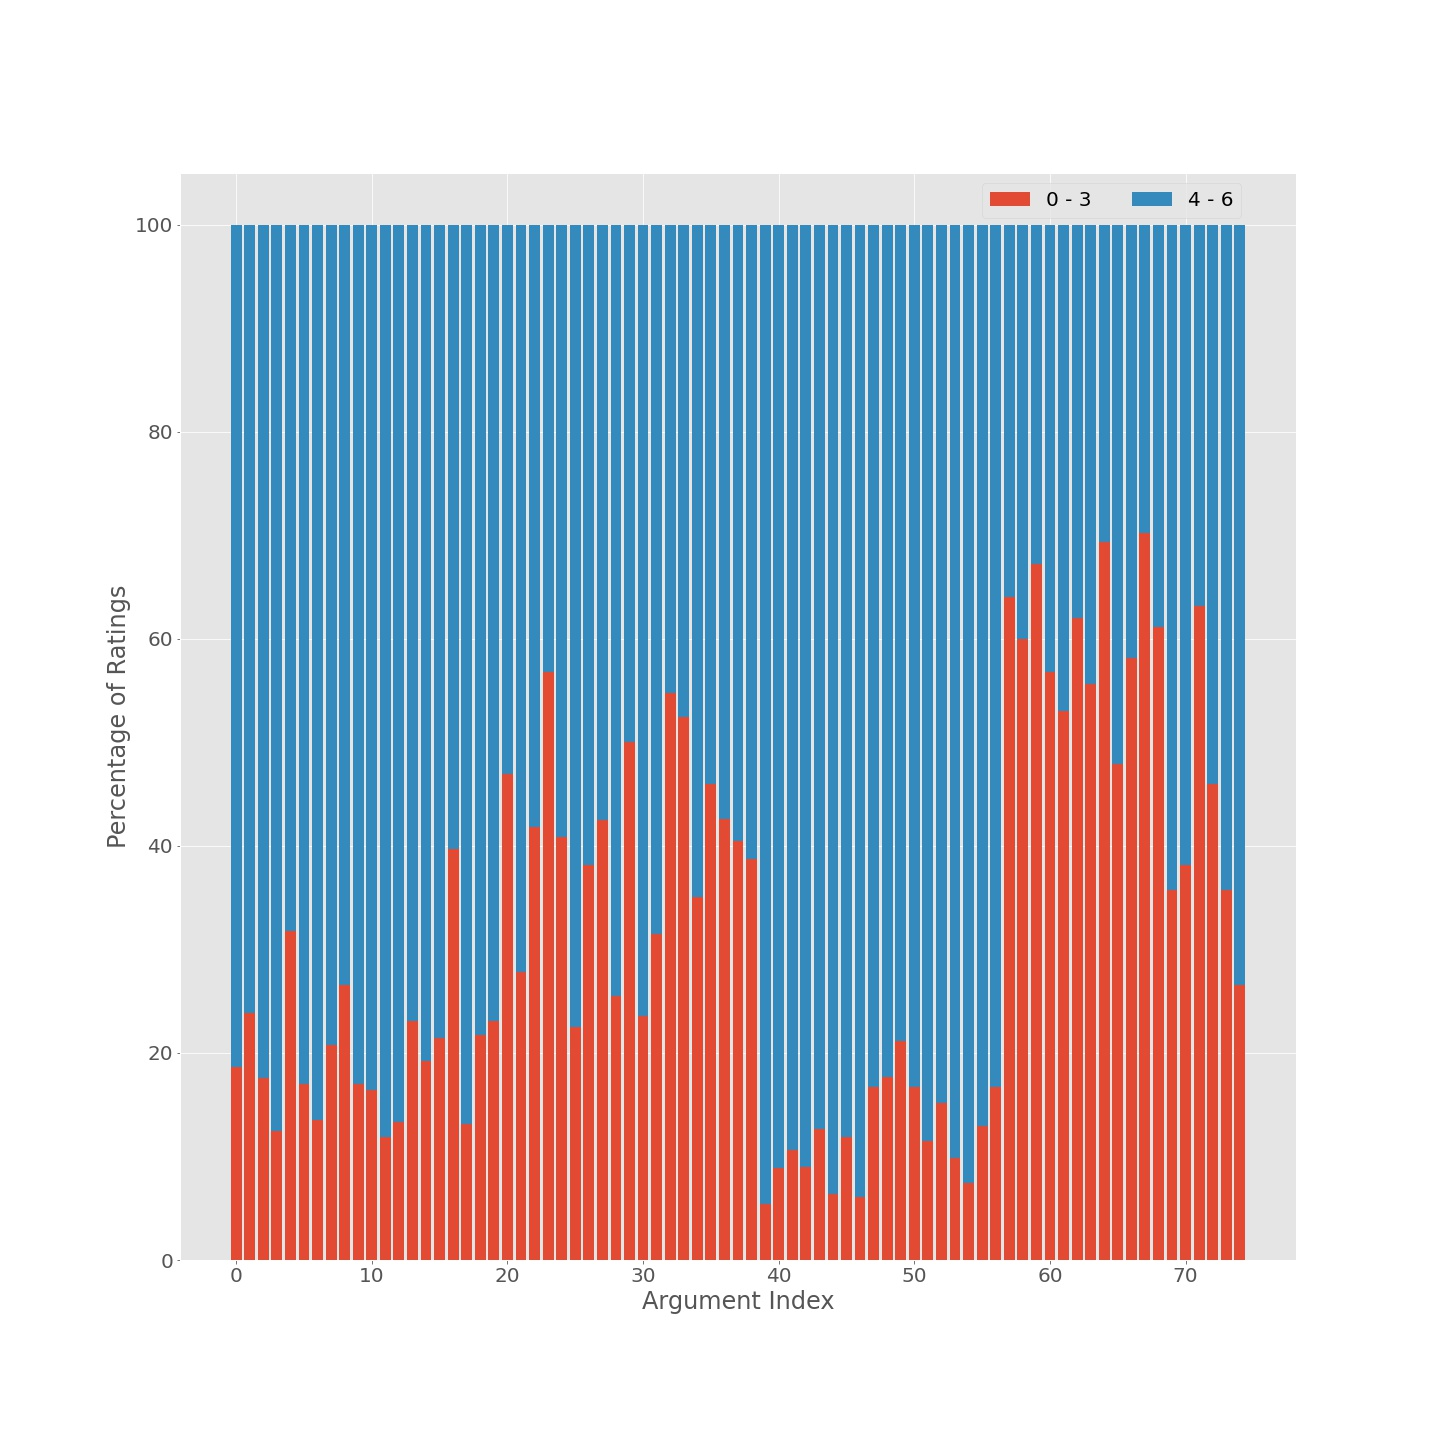
\includegraphics[width=1\textwidth]{images/T2_T3_train_Weight.jpg}
    \caption{Distribution of the Train – Ratings Given for Arguments in $T_2 \to T_3$ in Percentage for the Weight Task, Grouped by Rating Values 0 - 3 and 4 - 6.}
    \label{fig:conviction_t1_t2_train}
\end{figure}

\begin{figure}[!ht]
    \centering
    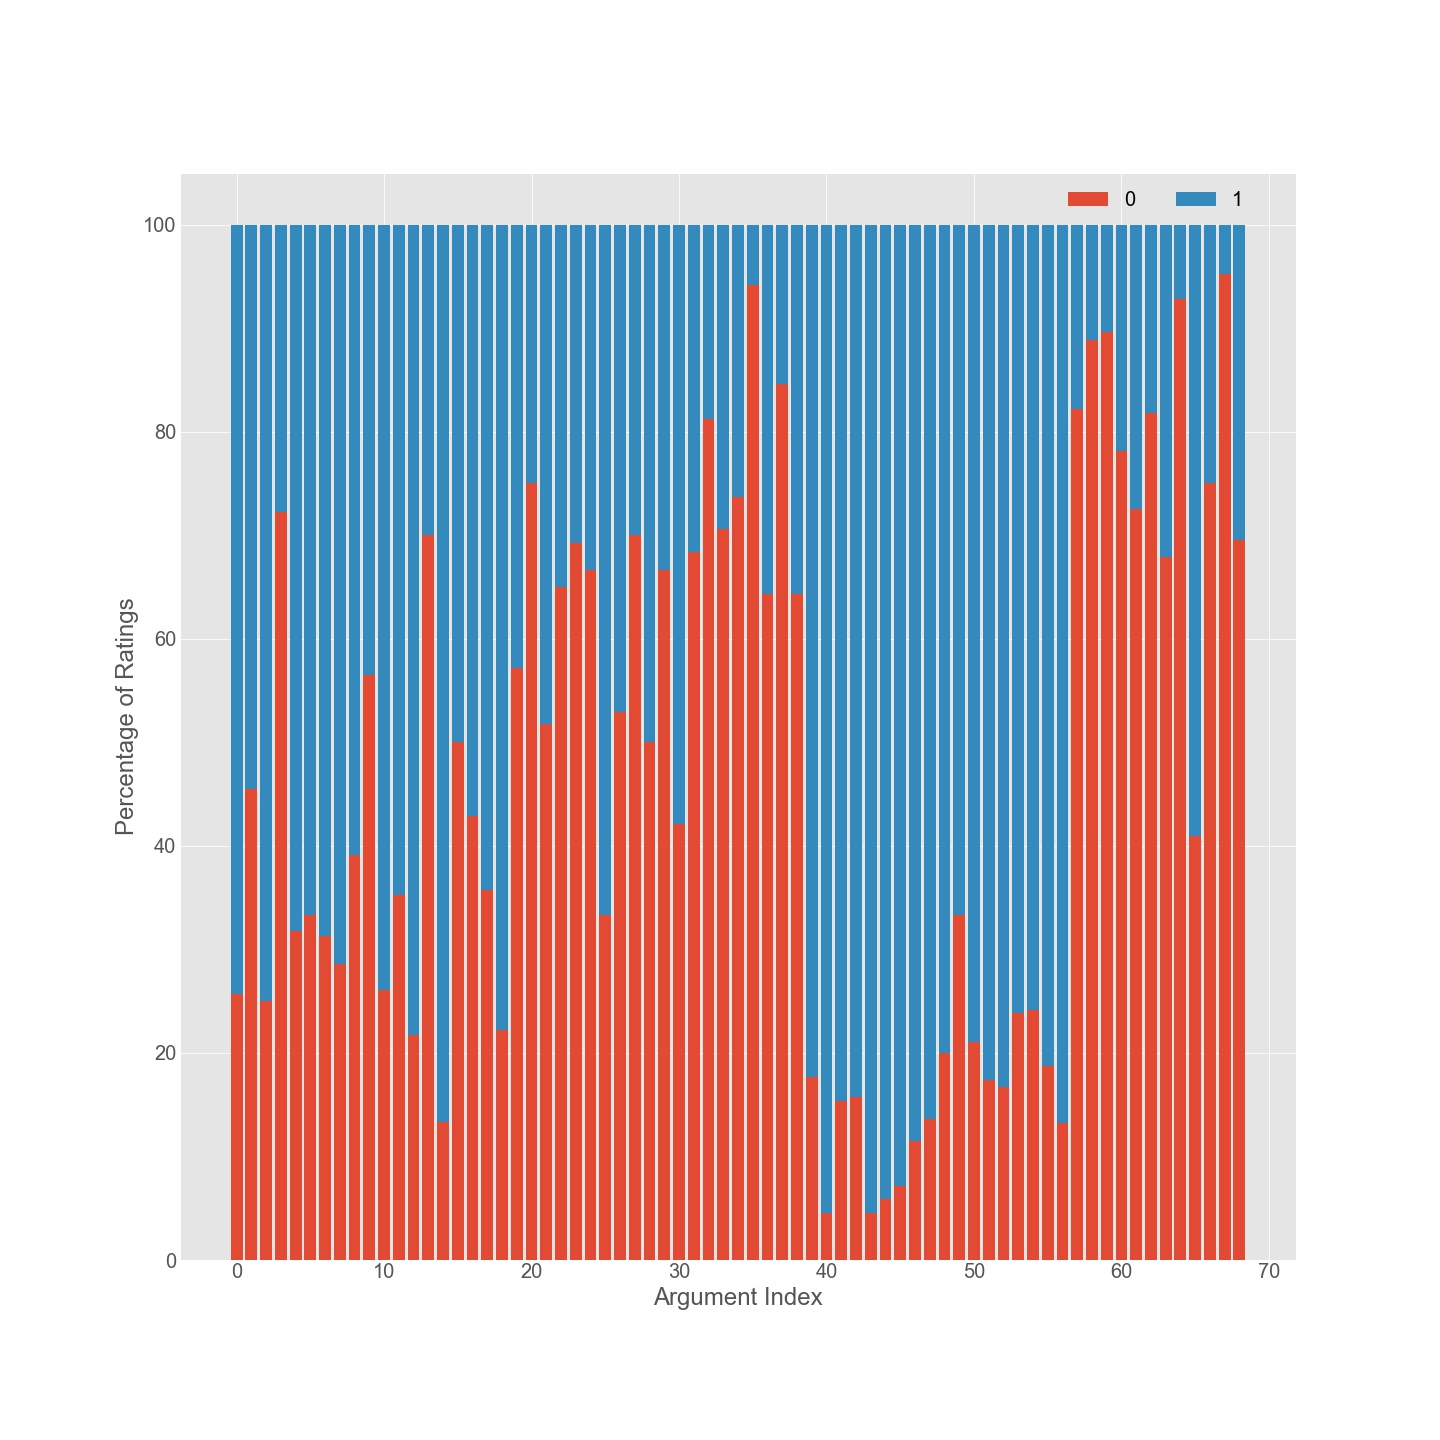
\includegraphics[width=1\textwidth]{images/T2_T3_test_Conviction.jpg}
    \caption{Distribution of the Test – Ratings Given for Arguments in $T_2 \to T_3$ in Percentage for the Conviction Task.}
    \label{fig:conviction_t2_t3_test}
\end{figure}

\begin{figure}[!ht]
    \centering
    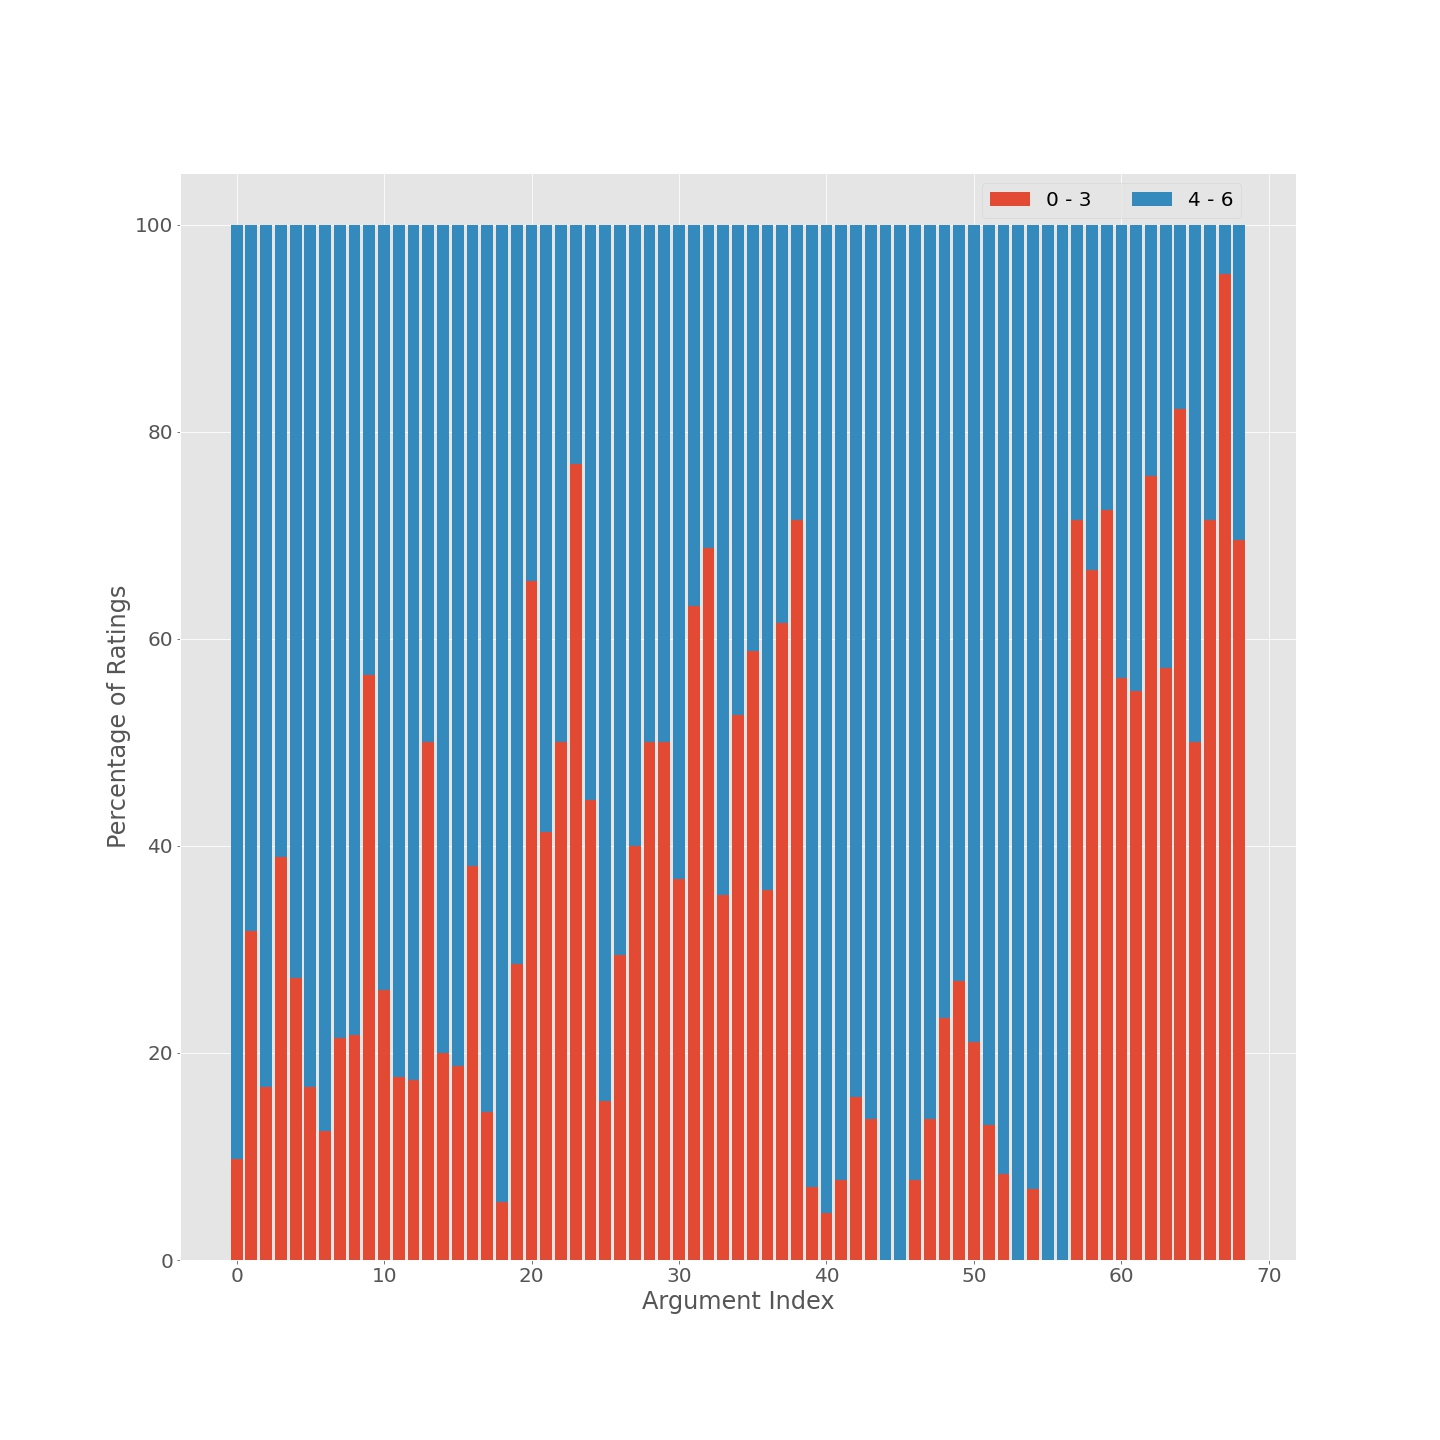
\includegraphics[width=1\textwidth]{images/T2_T3_test_Weight.jpg}
    \caption{Distribution of the Test – Ratings Given for Arguments in $T_2 \to T_3$ in Percentage for the Weight Task.}
    \label{fig:conviction_t2_t3_test}
\end{figure}